\documentclass[12pt]{report}
	\usepackage[margin=1in, top=1.5cm]{geometry}
	\usepackage[hidelinks, linktoc=all, pagebackref, russian]{hyperref}
	\usepackage{indentfirst}
    \usepackage{subcaption}
   	\usepackage[superscript,biblabel]{cite}
    \usepackage[font=small,labelfont=bf]{caption}
    \usepackage{abstract}
    \usepackage{mathtools}
    \usepackage{cleveref}
    \setlength{\parskip}{0.1cm}   
	\setlength{\parindent}{0.7cm}
    \usepackage{graphicx} % Used to insert images
    \usepackage{adjustbox} % Used to constrain images to a maximum size 
   	\usepackage{color} % Allow colors to be defined
    \usepackage{enumerate} % Needed for markdown enumerations to work
    \usepackage{geometry} % Used to adjust the document margins
    \usepackage{amsmath} % Equations
    \usepackage{amssymb} % Equations
    \usepackage[mathletters]{ucs} % Extended unicode (utf-8) support
    \usepackage[utf8x]{inputenc} % Allow utf-8 characters in the tex document
    \usepackage{fancyvrb} % verbatim replacement that allows latex
    \usepackage{grffile} % extends the file name processing of package graphics 
                         % to support a larger range 
    % The hyperref package gives us a pdf with properly built
    % internal navigation ('pdf bookmarks' for the table of contents,
    % internal cross-reference links, web links for URLs, etc.)
    \usepackage{longtable} % longtable support required by pandoc >1.10
\usepackage{bbm}

\newcommand{\diff}{\,\mathrm{d}} 	
 \renewcommand{\figureautorefname}{Fig.}%
\renewcommand*\thesection{\arabic{section}}
\DeclarePairedDelimiter\bra{\langle}{\rvert}
\DeclarePairedDelimiter\ket{\lvert}{\rangle}
\DeclarePairedDelimiterX\braket[2]{\langle}{\rangle}{#1 \delimsize\vert #2}
\newcommand{\rbrkt}[1]{\left( #1 \right)}
\newcommand{\sbrkt}[1]{\left[ #1 \right]}

\renewcommand*{\backreftwosep}{ and~}
\renewcommand*{\backreflastsep}{ and~}
\renewcommand*{\backref}[1]{}
\renewcommand*{\backrefalt}[4]{%
\ifcase #1 %
\relax%
\or
(referenced on p. [#2])%
\else
(referenced on p. [#2])%
\fi
}

\numberwithin{equation}{section}
\setcounter{tocdepth}{3}


\title{Reverse engineering of the Xmon qubits}

\graphicspath{{Pictures/}}

\begin{document}
\maketitle
\tableofcontents

\chapter{Resonator-feedline coupling}

\section{Equations for quality factors}

The observed quality factor of a microwave transmission line resonator (TLR) $Q_l$ (loaded quality factor) can be calculated as a sum of two parts -- the internal and external quality factors. The internal quality factor $Q_i$ describes how excitations leave the resonator in the absence of coupling to the transmission line, so damping in this case comes from the internal defects of the resonator itself. When, however, the resonator is coupled to the external circuitry with some active resistance, the damping is enhanced and the observed Q-factor is reduced according to the following formula:
\begin{equation}
Q_l^{-1} = Q_i^{-1}+Q_e^{-1},
\label{eq:qfactor}
\end{equation}
where $Q_e$ is determined by the value of the externally connected resistance and the way of its connection.

\begin{figure}
\captionsetup[subfigure]{width = 0.9\textwidth, justification=normal}
\centering
\begin{subfigure}[t]{0.48\textwidth}
\centering
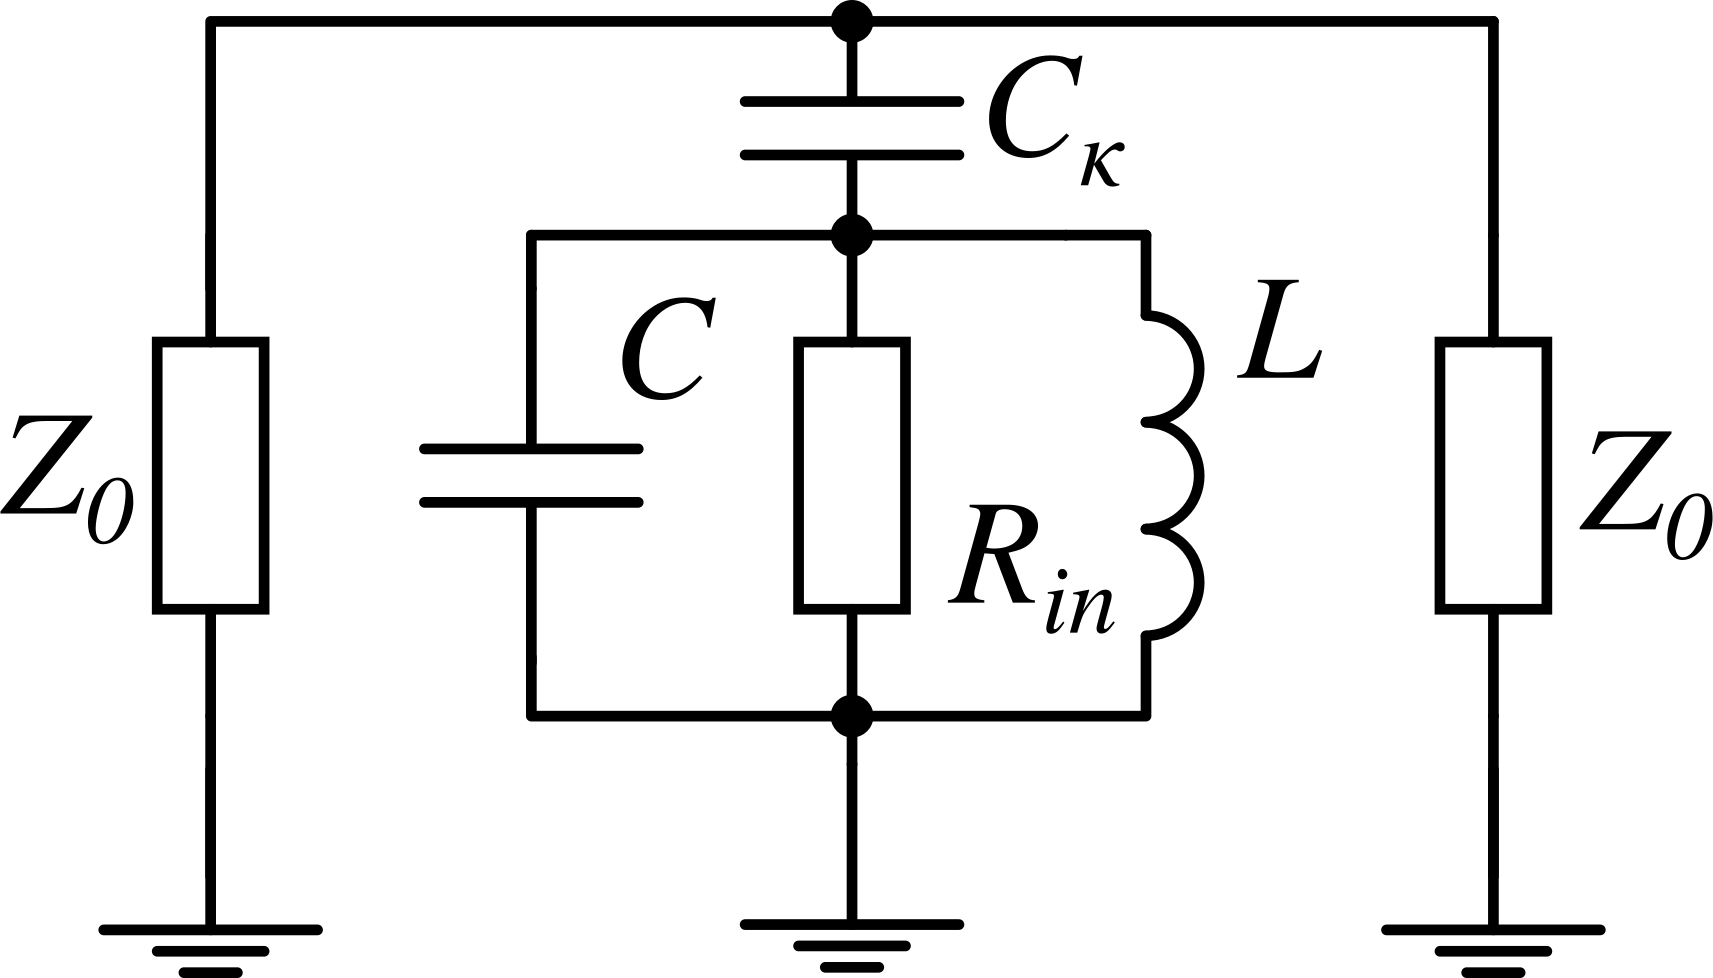
\includegraphics[width=0.9\textwidth]{resonator}
\caption{Real world circuit configuration.}
\end{subfigure}
\begin{subfigure}[t]{0.48\textwidth}
\centering
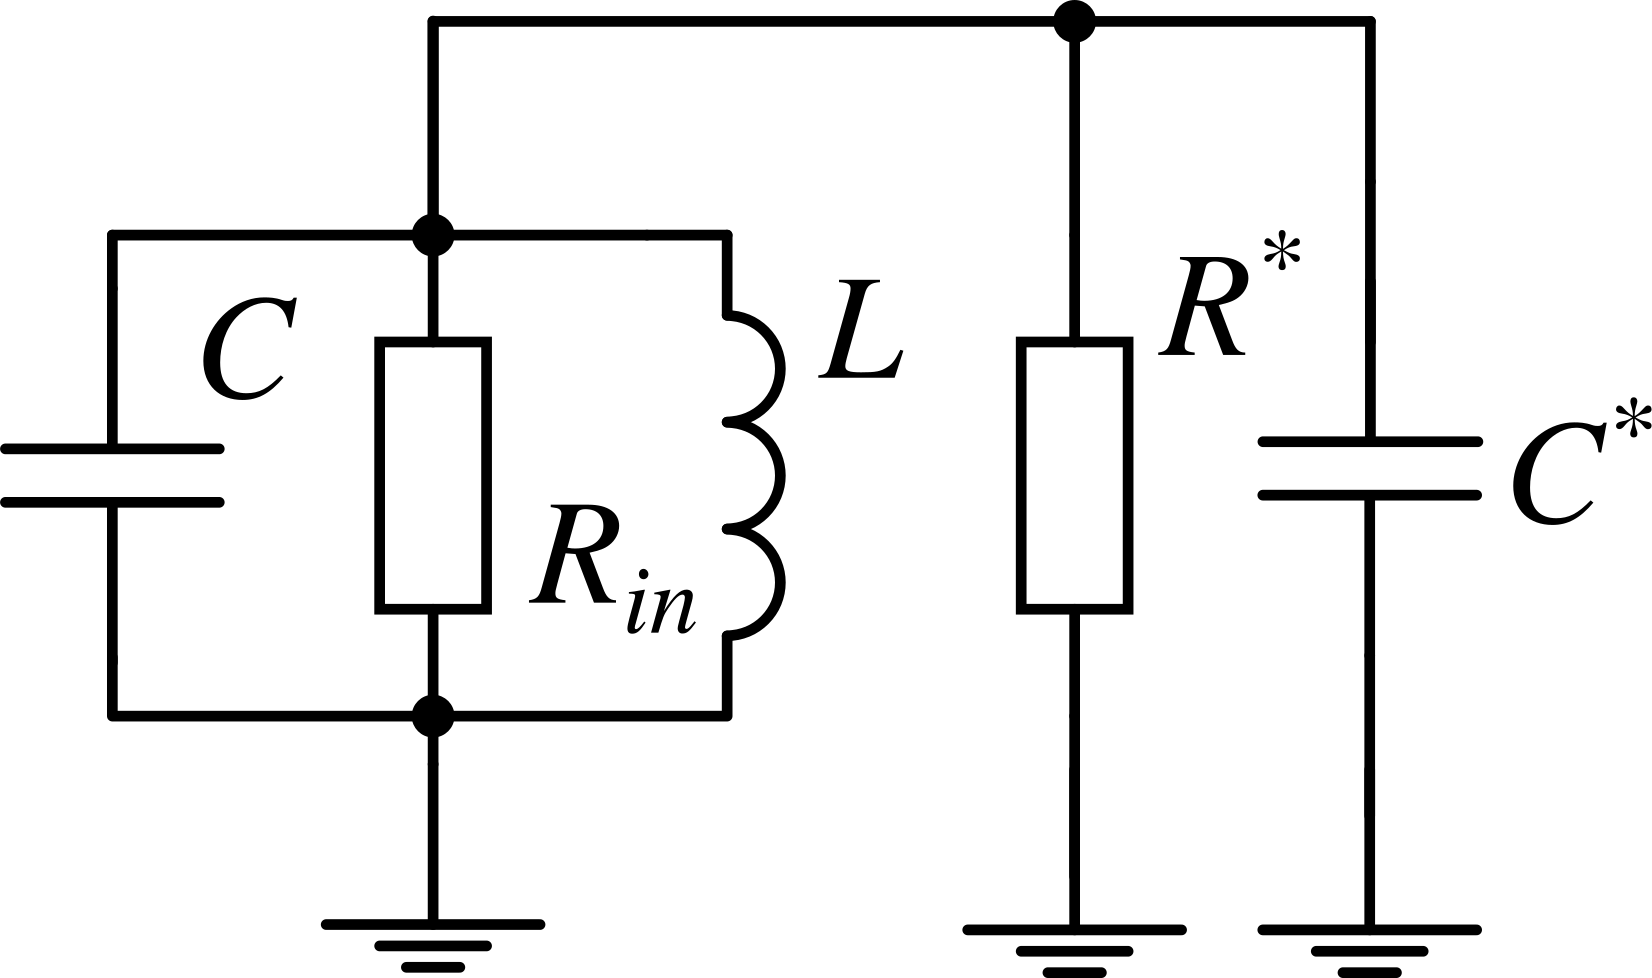
\includegraphics[width=0.9\textwidth]{resonator_equiv}
\caption{Norton equivalent of (a).}
\end{subfigure}

\caption{Equivalent circuit for a $\lambda/4$ TLR, capacitively coupled to the transmission line from the system's point of view.}
\label{fig:resonator_equiv}
\end{figure}

The common way of connection is the capacitive coupling $C_\kappa$ to the transmission line, as depicted on the equivalent scheme of the circuit in \autoref{fig:resonator_equiv}~(a). To draw the equivalent scheme of the circuit one needs first to determine the type of the resonance for the chosen TLR\cite{pozar2012}. In the studied design the resonators are $\lambda/4$ thus the equivalent for each of them is the parallel RLC resonator, where $C$ and $L$ are equivalent capacitance and inductance and $R=R_{in}$ characterises the internal dissipation. Its $Q_i  = \omega_0	C R_{in}$ where $\omega_0 = \sqrt{1/LC}$ can be calculated from the definition when no external impedance is connected.
 
The external Q-factor can be derived in a bit more complicated way\cite{Goppl2008}. We can transform the circuit on the \autoref{fig:resonator_equiv}~(a) to explicitly include the external parameters in the internal ones. To do so one needs to convert the series connection of the coupling capacitor and the characteristic impedances into parallel, as done on the \autoref{fig:resonator_equiv}~(b). The $R^*$ and $C^*$ impedances should be chosen in such a way that total impedance of the external circuit was the same as before the transformation. To achieve this $R^*$ and $C^*$ must be calculated as follows:
\begin{gather}
R^{*} = \frac{1+\omega^2 C_\kappa^2 (Z_0/2)^2}{\omega^2 C_\kappa^2 (Z_0/2)	}, \\
C^{*} = \frac{C_\kappa}{1+\omega^2 C_\kappa^2 (Z_0/2)^2} \approx C_\kappa (\text{for our case}). \label{eq:C_ast}
\end{gather}
From this and \autoref{fig:resonator_equiv}~(b) it is simple to write down the expression for the external and loaded quality factors:
\begin{gather}
Q_e = \omega (C+C^{*}) R^{*}, \\
Q_l = \omega (C+C^{*})  \frac{1}{1/R^{*}+1/R_{in}}. \label{eq:Q_l}
\end{gather}
If one considers $C^{*} \ll C$ the above expressions readily justify \eqref{eq:qfactor}. The values been used in the simulations are: $C = 350$ fF, $L = 2$ nH, $R_{in}=10^7$ Ohm, $Z_0 = 50$ Ohm.

\begin{figure}
\centering
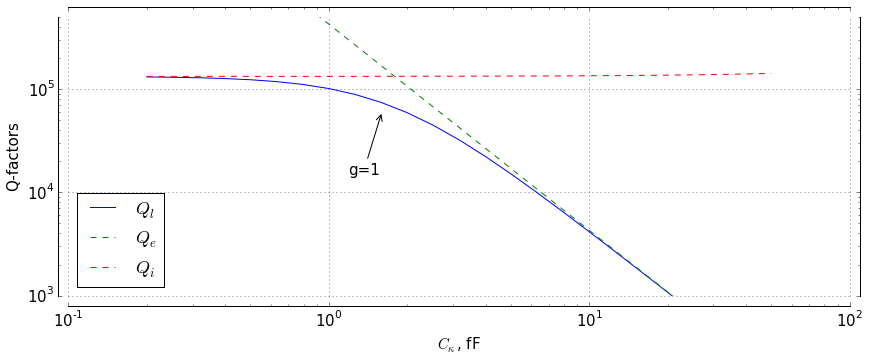
\includegraphics[width=0.9\textwidth]{q-factors}
\caption{Q-factors dependence on $C_\kappa$ according to \eqref{eq:Q_l}.}
\end{figure}



\begin{figure}
\centering
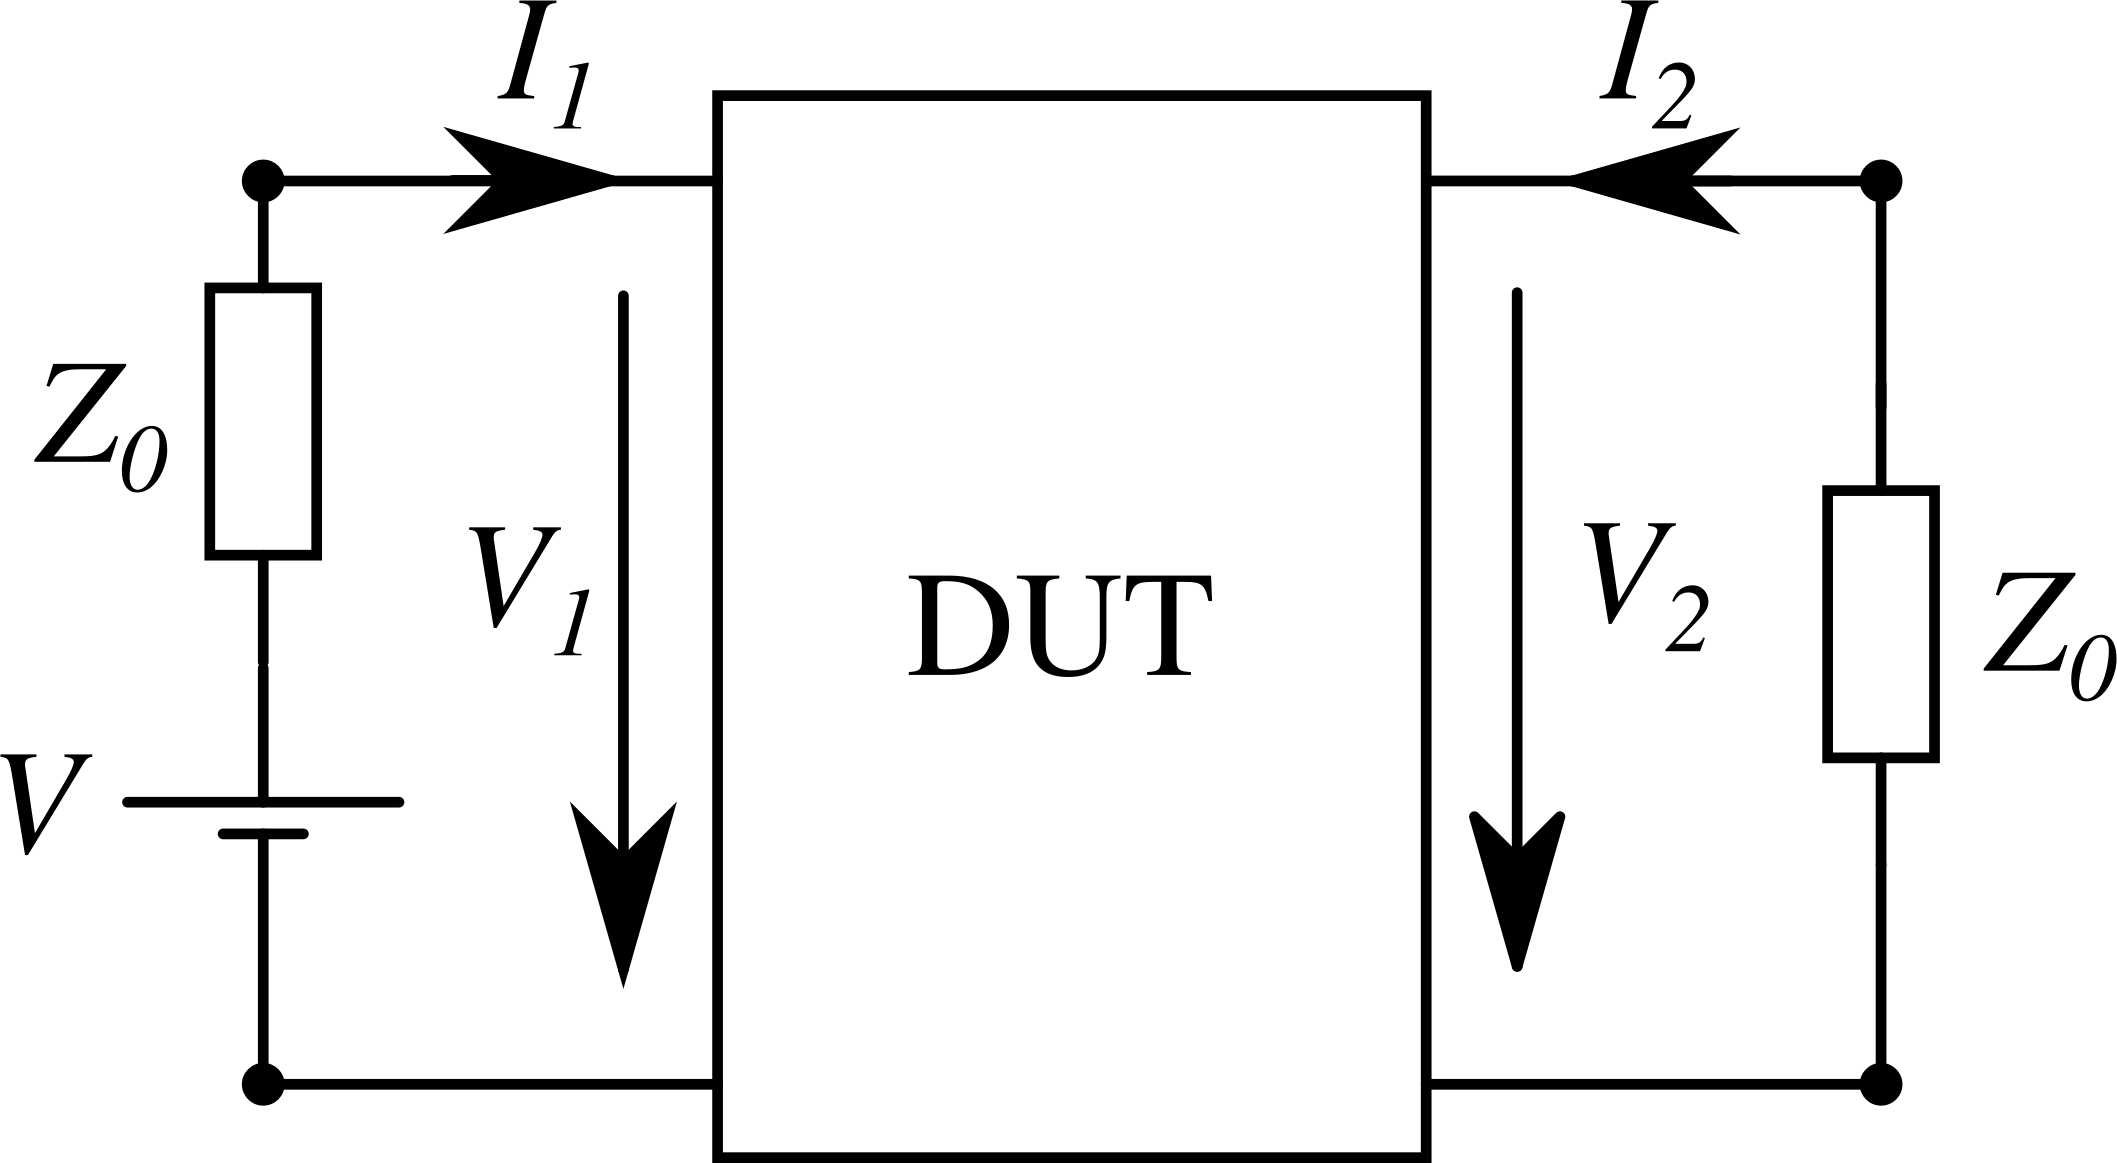
\includegraphics[width=0.5\textwidth]{tl_scheme_general}
\caption{A scheme for the two-port network.}
\label{fgeneral2port}
\end{figure}

\section{S-parameters}

\subsection{Introduction}

In the following two subsections we will discuss the scattering matrix for the two different configurations of resonator coupling. Generally, a two-port microwave device under test can be drawn like in \autoref{fgeneral2port}. For such system it is possible to calculate different 2 by 2 matrices, which bind together voltages and currents on the ports 1 and 2.

To calculate S-parameters one needs to treat voltages and currents, which can be calculated from Kirchhoff's laws, as a sum of the incident and reflected components (``+'' corresponds to the incident wave and ``$-$'' to the reflected wave):
\begin{gather*}
V_{1,2} = V_{1,2}^+ + V_{1,2}^- ,\\
I_{1,2} = I_{1,2}^+ + I_{1,2}^- = \frac{ V_{1,2}^+ - V_{1,2}^- }{Z_0},
\end{gather*}
where the difference in the second expression arises from telegrapher's equations. Solving these with respect to incident and reflected components, one can get
\begin{equation*}
V_{1,2}^\pm = \frac{1}{2}(V_{1,2} \pm Z_0 I_{1,2}).
\end{equation*}
From this, finally, S-parameters are defined:
\begin{equation}
\rbrkt{\begin{matrix}
V_1^- \\
V_2^-
\end{matrix}} = 
\rbrkt{\begin{matrix}
S_{11} & S_{12} \\
S_{21} & S_{22}
\end{matrix}}
\rbrkt{\begin{matrix}
V_1^+ \\
V_2^+
\end{matrix}}.
\label{eq:S_def}
\end{equation}
However, it's often more convenient to use indirect methods of calculating S-parameters, for example, to extract them from $ABCD$-matrix.

\subsection{Coupled (shunting) design}
For a coupled design one can treat the resonator as a shunt in the transmission line as in \autoref{fig:shunted_tl}. Except by the definition \eqref{eq:S_def} there are two other ways to calculate the S-matrix. First one is intuitive but is not valid for every configuration. Transmission and reflection parameters are defined\cite{Kiselev2013} below (the second formula is valid only for the ``shunt'' configuration, no series elements are allowed in the line):
\begin{gather}    
\Gamma = \frac{Z_{eff} - Z_{0}}{Z_{eff} + Z_{0}} = S_{11} = S_{22}, \label{eGamma}\\
T = \frac{2Z_{eff}}{Z_{eff}+Z_0} \overset{!}{=} S_{21} = S_{12}, \label{eT}
\end{gather}
where $Z_{eff} = Z_0 || Z_{shunt}$ and the equalities between S-parameters hold due to the symmetry.\begin{figure}[h]
\centering
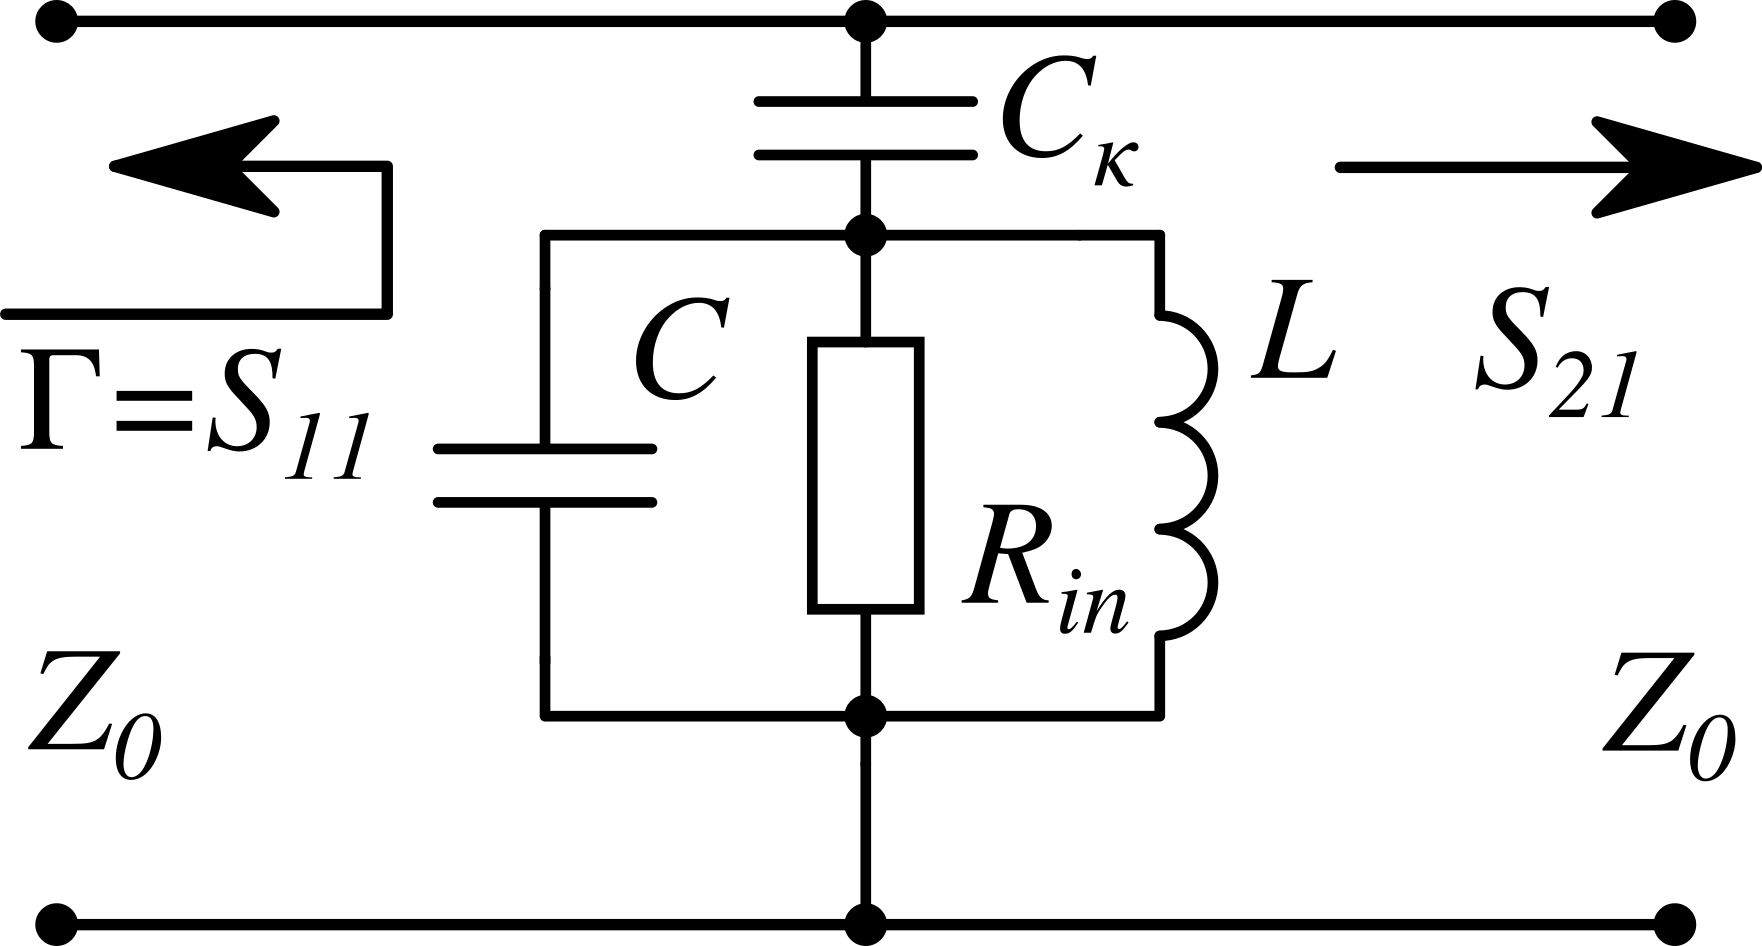
\includegraphics[width=0.5\textwidth]{tl_scheme}
\caption{The shunted transmission line. This is \autoref{fig:resonator_equiv}~(a)  from the observer's point of view.}
\label{fig:shunted_tl}
\end{figure}
\begin{figure}[h]
\centering
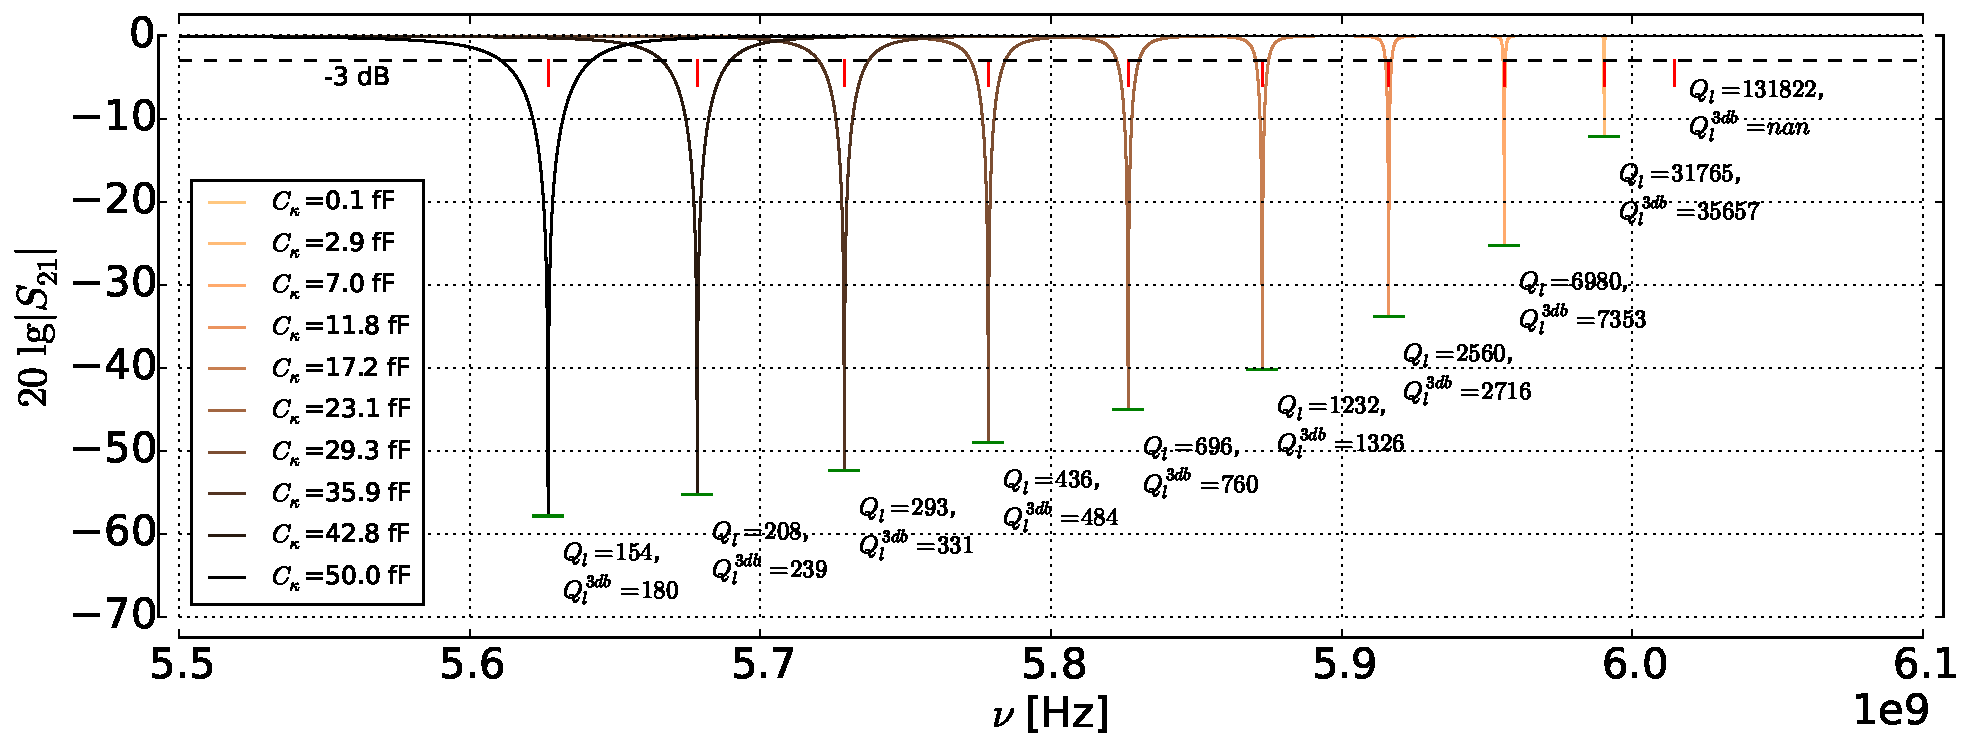
\includegraphics[width=0.99\textwidth]{S21s}
\caption{ $S_{21}$ parameters simulated with \eqref{eq:S21} for different coupling strengths. The loaded quality factors are calculated with \eqref{eq:Q_l} and with ``3db''-method. The red dashes show the values of expression $\sqrt{1/L(C+C_k)}$ according to \autoref{fig:resonator_equiv}~(b), the green ones show the theoretically predicted depths.}
\label{fig:S21s}
\end{figure}

Another way is to calculate $ABCD$ matrix or impedance matrix and convert it to the S-matrix with corresponding formulae\cite{pozar2012}. In the ``shunted'' case from both this approaches the simplified expressions for the S-parameters follow:
\begin{gather}
S_{11} = -\frac{Z_0}{1 + 2Z_{shunt}/Z_0} = S_{22}, \\
S_{21} = \frac{1}{1+Z_0/2Z_{shunt}} = S_{12}. \label{eq:S21}
\end{gather}
The second expression is plotted in \autoref{fig:S21s} along with the loaded quality factors calculated by \eqref{eq:Q_l} and by ``3db''-method. It can be seen that with increase of capacitance resonance frequency shifts down, which is expected according to \autoref{fig:resonator_equiv}~(b) and \eqref{eq:C_ast} and $Q_l$ decreases.

In \autoref{fig:S21s} the resonance frequencies calculated from the equivalent circuit in \autoref{fig:resonator_equiv}~(b) are shown along with the analytically calculated depths of the peaks:
\begin{equation}
\min_f S_{21} = \frac{2 L \left(C + C_{\kappa}\right)}{\sqrt{C_{\kappa}^{2} L Z_{0}^{2} \left(C + C_{\kappa}\right) + \left(2 (C+C_\kappa) L + C_{k}^{2} R_{in} Z_{0} \right)^{2}}}.
\end{equation}

\subsection{Embedded (series) design}

For the embedded resonator it's possible to draw a similar equivalent circuit as for the ``shunt'' design\cite{Goppl2008}. It is depicted in \autoref{fseries_tl}. 

\begin{figure}[h]
\centering
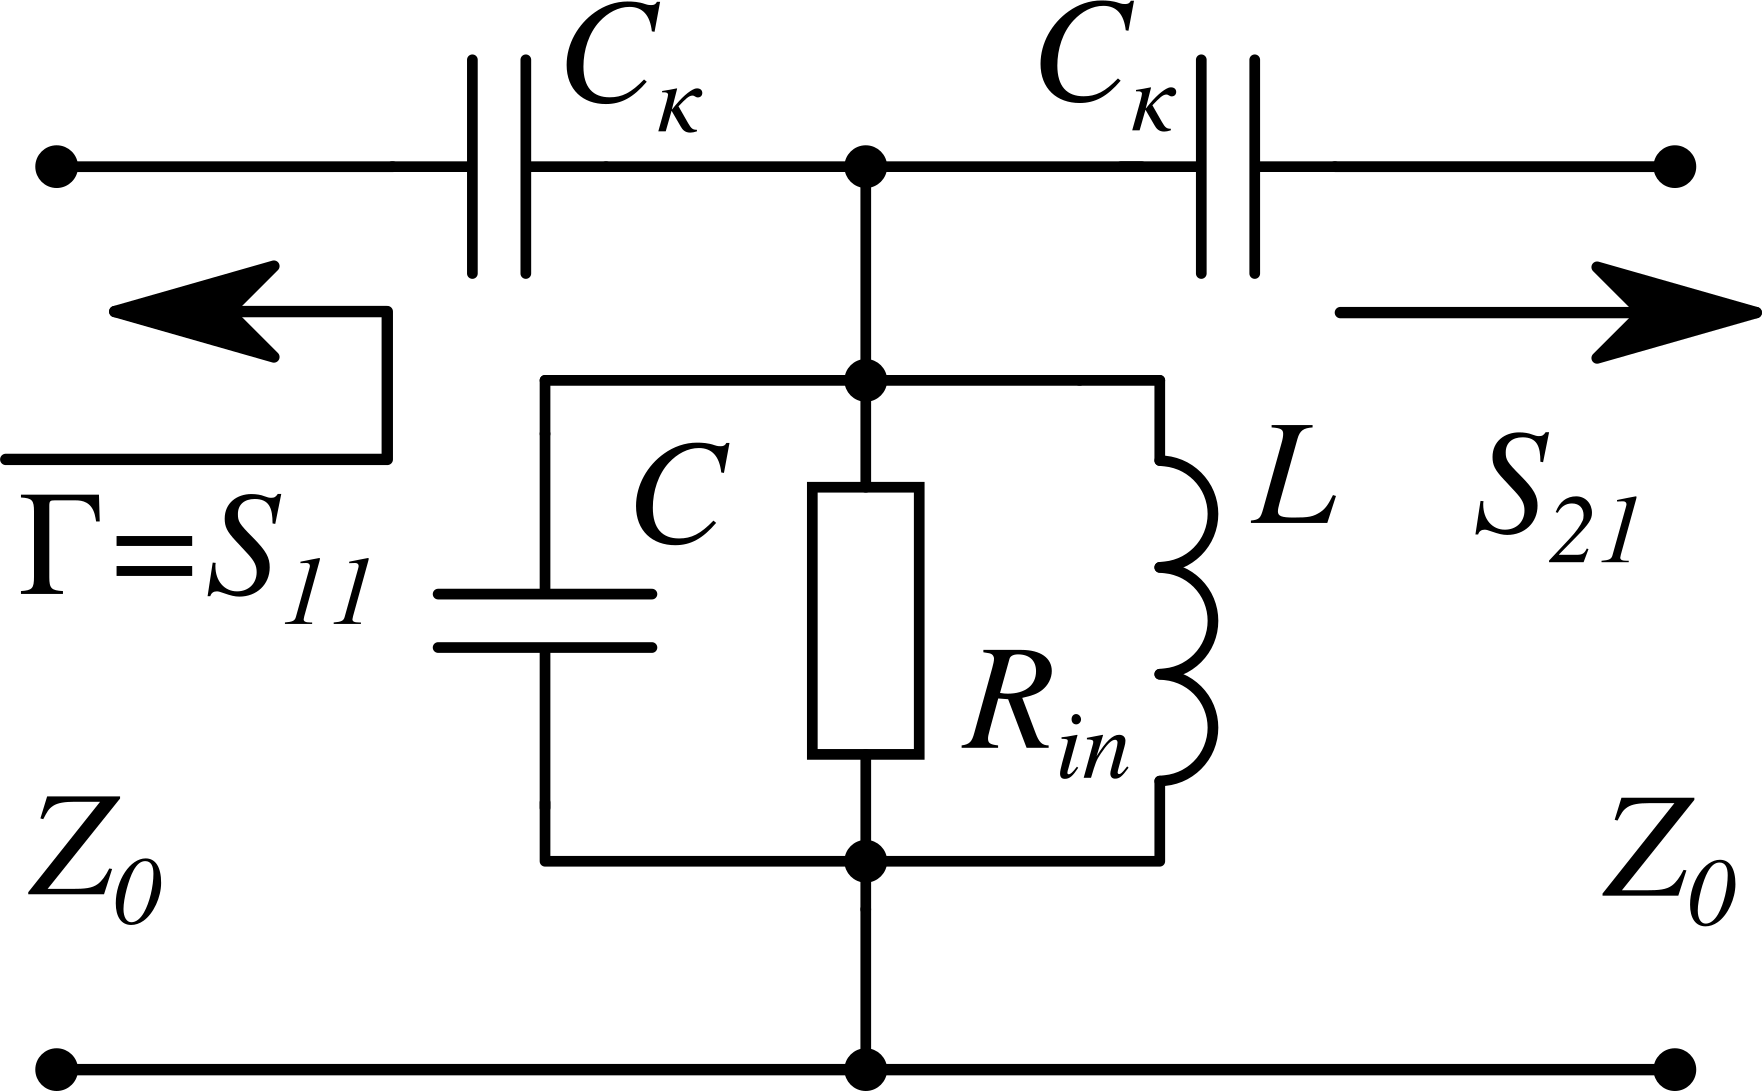
\includegraphics[width=0.5\textwidth]{tl_scheme_series}
\caption{The equivalent circuit for the embedded resonator.}
\label{fseries_tl}
\end{figure}
\begin{figure}[h]
\centering
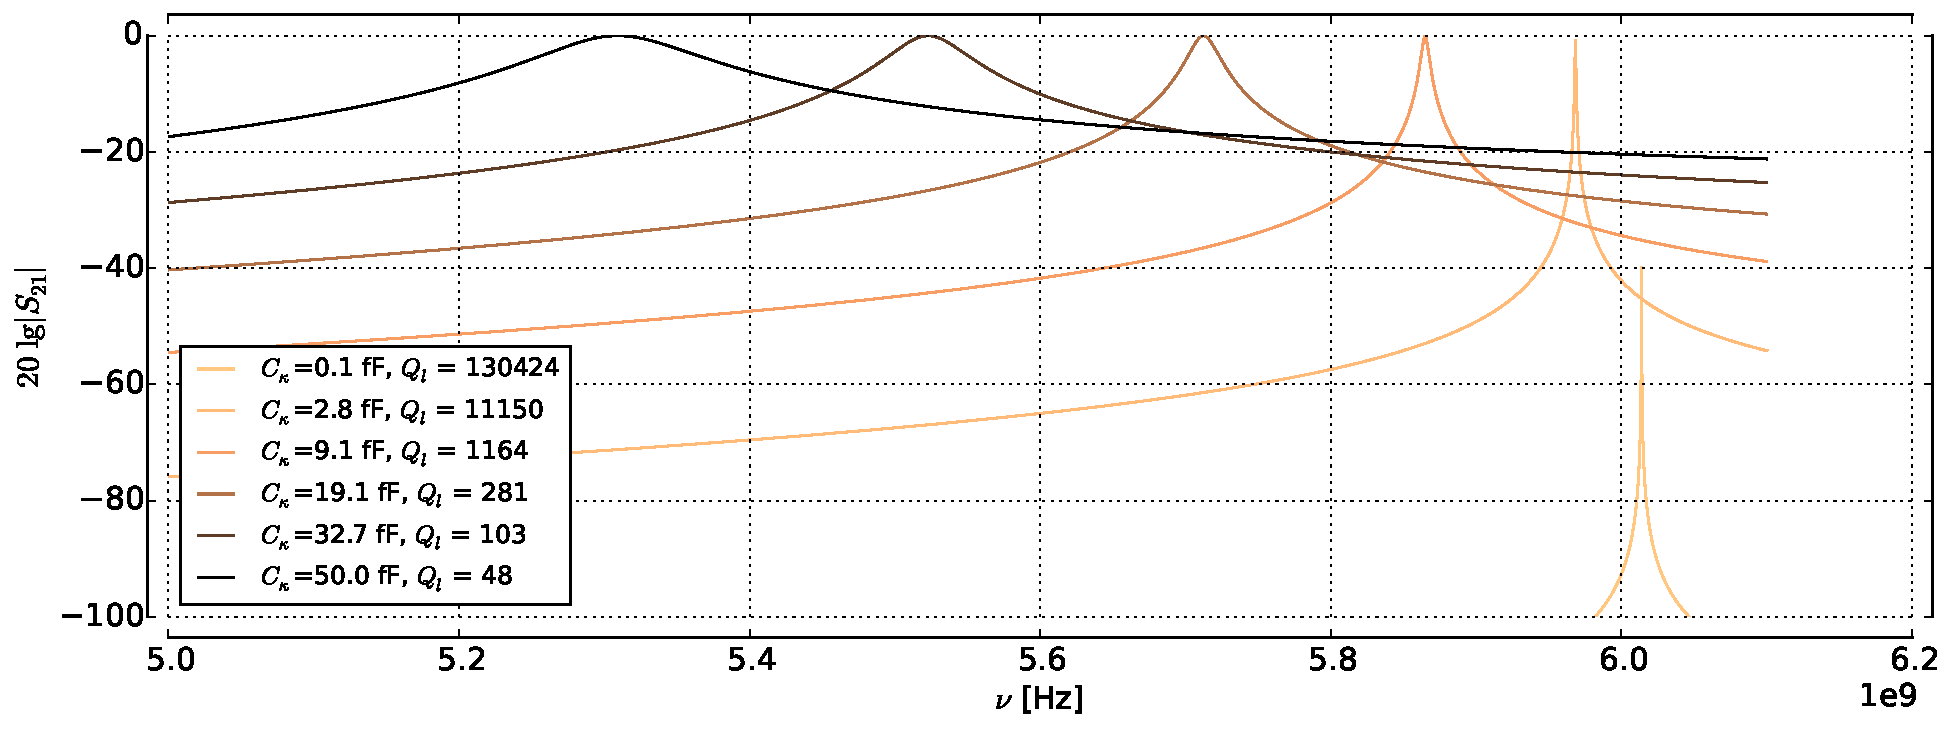
\includegraphics[width=0.9\textwidth]{S21s_series}
\caption{$S_{21}$ for the series configuration. Loaded Q-factors were calculated  via analytic expression similar to \eqref{eq:Q_l}.}
\label{fS21s_series}
\end{figure}

For this kind of connection of the resonator to the transmission line \eqref{eT} is now not valid (however, \eqref{eGamma} still holds true). To calculate transmission in this case one can find the transmission matrix and then convert it to the S-matrix or use Kirchhoff's laws and \eqref{eq:S_def}. For studied case one can get the following $ABCD$-matrix\cite{pozar2012}
\begin{equation}
\hat T = \rbrkt{\begin{matrix}
A & B \\
C & D
\end{matrix}} = \rbrkt{\begin{matrix}
1 + \frac{1/i\omega C_\kappa}{Z_{res}} & 2/i\omega C_\kappa - \frac{\omega^2 C_\kappa^2}{Z_{res}} \\
1/Z_{res} &  1 + \frac{1/i\omega C_\kappa}{Z_{res}} 
\end{matrix}},
\end{equation}
where $Z_{res} = R_{in}||i\omega L || 1/i\omega C$. The corresponding $S_{21}$ is  plotted in \autoref{fS21s_series} and can be calculated as\cite{pozar2012} 
\begin{equation}
S_{21} = \frac{2}{A+B/Z_0 +CZ_0 + D}.
\end{equation}

\chapter{Xmon-resonator coupling}

\begin{figure}
\centering
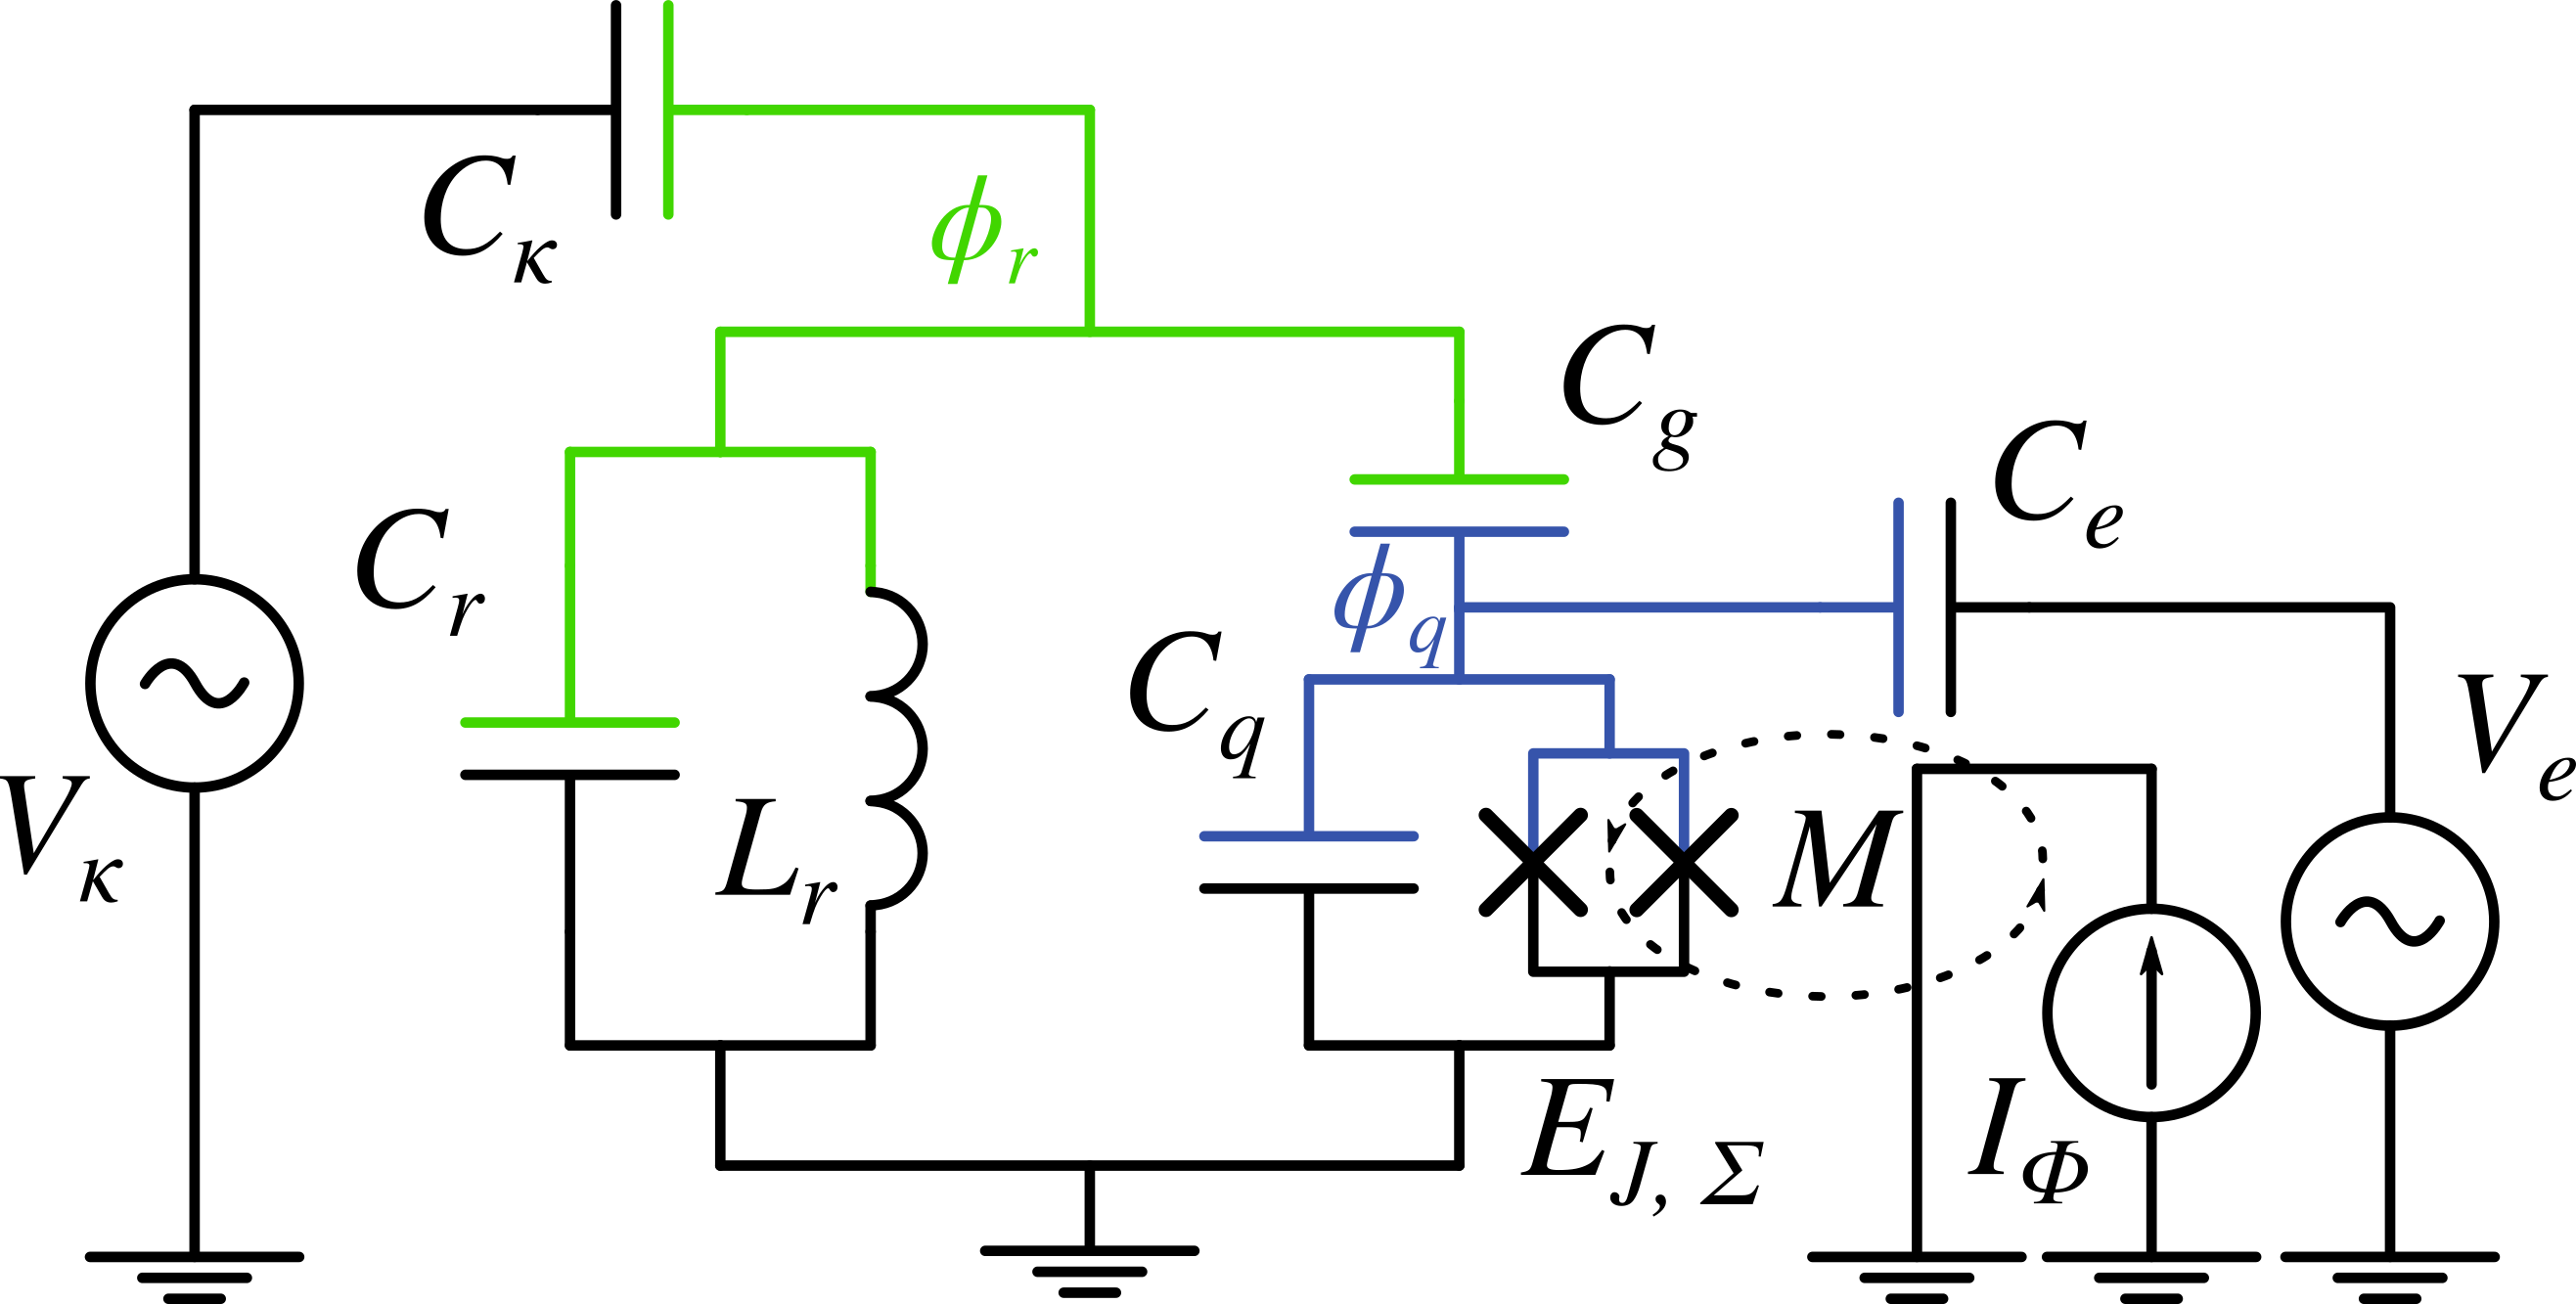
\includegraphics[width=0.8\textwidth]{xmon_resonator}
\caption{Equivalent circuit for coupled system of a tunable transmon qubit and a resonator. Colors show nodes (or branches) containing system's degrees of freedom according to M. Devoret's theory\cite{Devoret1995}.}
\label{fig:xmon-resonator}
\end{figure}
\begin{figure}
\centering
\begin{subfigure}[t]{\textwidth}
\centering
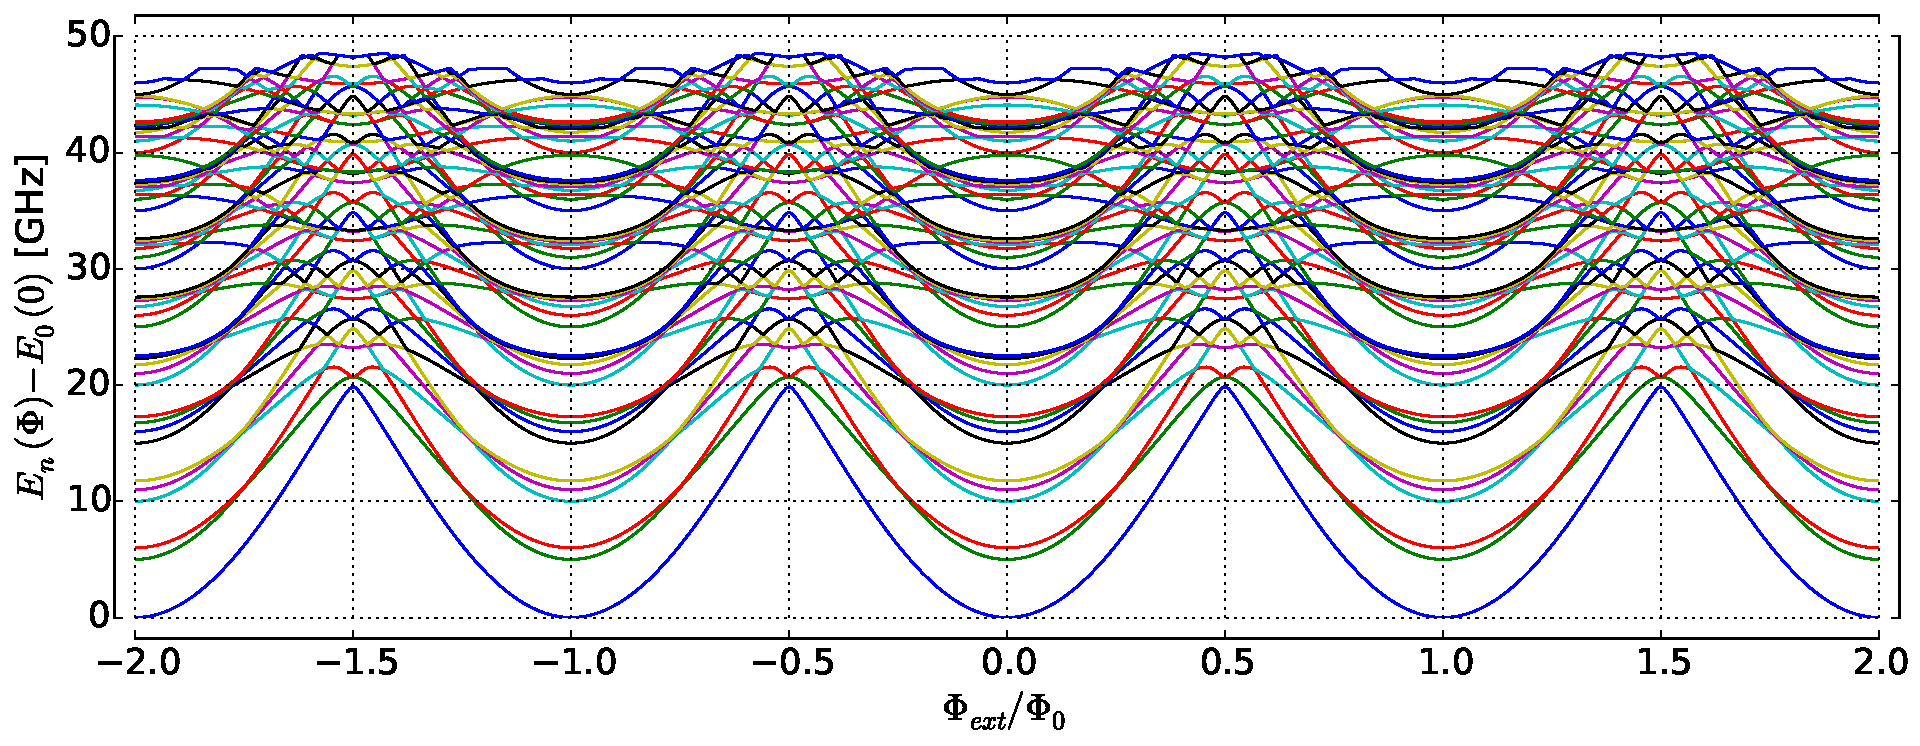
\includegraphics[width=0.9\textwidth]{levels}
\end{subfigure}

\begin{subfigure}[t]{\textwidth}
\centering
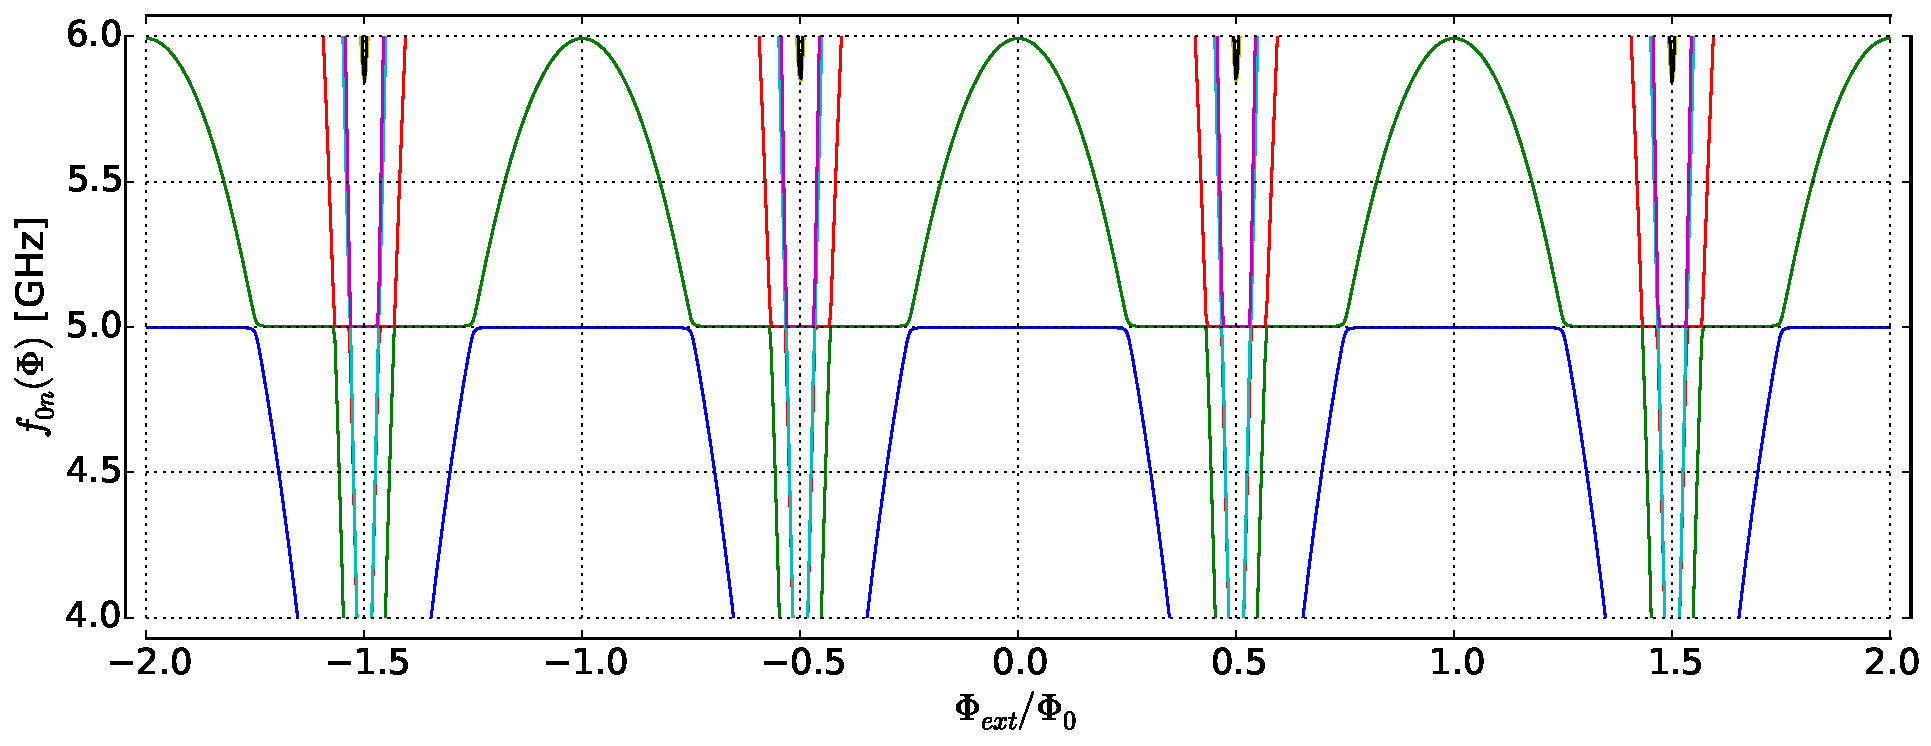
\includegraphics[width=0.9\textwidth]{freqs}
\end{subfigure}
\caption{Energy structure of the studied system depending on $\Phi_{ext}$.}
\label{fig:levels}
\end{figure}
\section{Hamiltonian for the compound system}

Here we will use the results acquired by Bader\cite{Bader2013} and Koch\cite{Koch2007}. Using \autoref{fig:xmon-resonator} it is possible to obtain the quantized Hamiltonian for the compound circuit:

\begin{equation}
\begin{gathered}
\mathcal{\hat H} =  \underbrace{\frac{\hat \phi_r^2}{2 L_r} + \frac{(C_q+C_g) \hat Q_r^2}{2C_*^2}}_\text{resonator} 
+ \underbrace{\frac{(C_g + C_\kappa + C_r) \hat Q^2_q}{2C_*^2} - E_J (\Phi_{ext}) \cos \frac{2e}{\hbar}\hat \phi_q }_\text{qubit}
+ \underbrace{\frac{C_g\hat Q_r \hat Q_q}{C_*^2}}_\text{coupling} = \\
=  \hbar\omega_r\ \hat a^\dag \hat a \otimes \mathbbm{\hat 1}_q \quad (\mathcal{\hat H}_r) \\
+ 4 E_C\ \mathbbm{\hat 1}_r \otimes \hat n^2 - \frac{E_J(\Phi_{ext})}{2}\ \mathbbm{\hat 1}_r\otimes \sum_{n=-\infty}^{+\infty} \ket{n+1}\bra{n} + \ket{n}\bra{n+1} \quad (\mathcal{\hat H}_q) \\
- 2e \frac{C_g}{C_*} \sqrt{\frac{\hbar \omega_r }{2(C_q+C_g)}}\ i(\hat a^\dag - \hat a) \otimes \hat n, \quad (\mathcal{\hat H}_i)
\end{gathered}\label{eq:hamiltonian}
\end{equation}
where 
$$C_*^2 = C_q C_g + C_q C_\kappa + C_g C_\kappa + C_q C_r + C_g C_r, $$
$$\omega_r = 1/\sqrt{L_r C_*^2/(C_q+C_g)}, $$
$$E_C = \frac{(C_g+C_\kappa+C_r)e^2}{C_*^2}, $$
$$E_J(\Phi_{ext}) = E_{J,\Sigma} \cos(\Phi_{ext}/\Phi_0),\ \Phi_{ext} = I_\Phi M.$$
Presuming the coupling is not very strong ($C_g \ll C_q, C_r$) it is possible also to include simple time-dependent driving terms for both subsystems:
\begin{gather}
\mathcal{\hat H}_r^d(t) = \frac{C_\kappa V_\kappa(t)}{C_r + C_\kappa} \hat Q_r \propto f_r(t)\ i(\hat a^\dag - \hat a) \otimes \mathbbm{\hat 1}_q, \notag \\
\mathcal{\hat H}_q^d(t) = \frac{C_e V_e(t)}{C_q + C_e} \hat Q_q \propto f_q(t)\  \mathbbm{\hat 1}_r \otimes \hat n,
\label{eq:driving_q}
\end{gather}
where $f_{q, r} (t)$ are the effective values of the drive magnitude at time $t$.

\begin{figure}
\centering
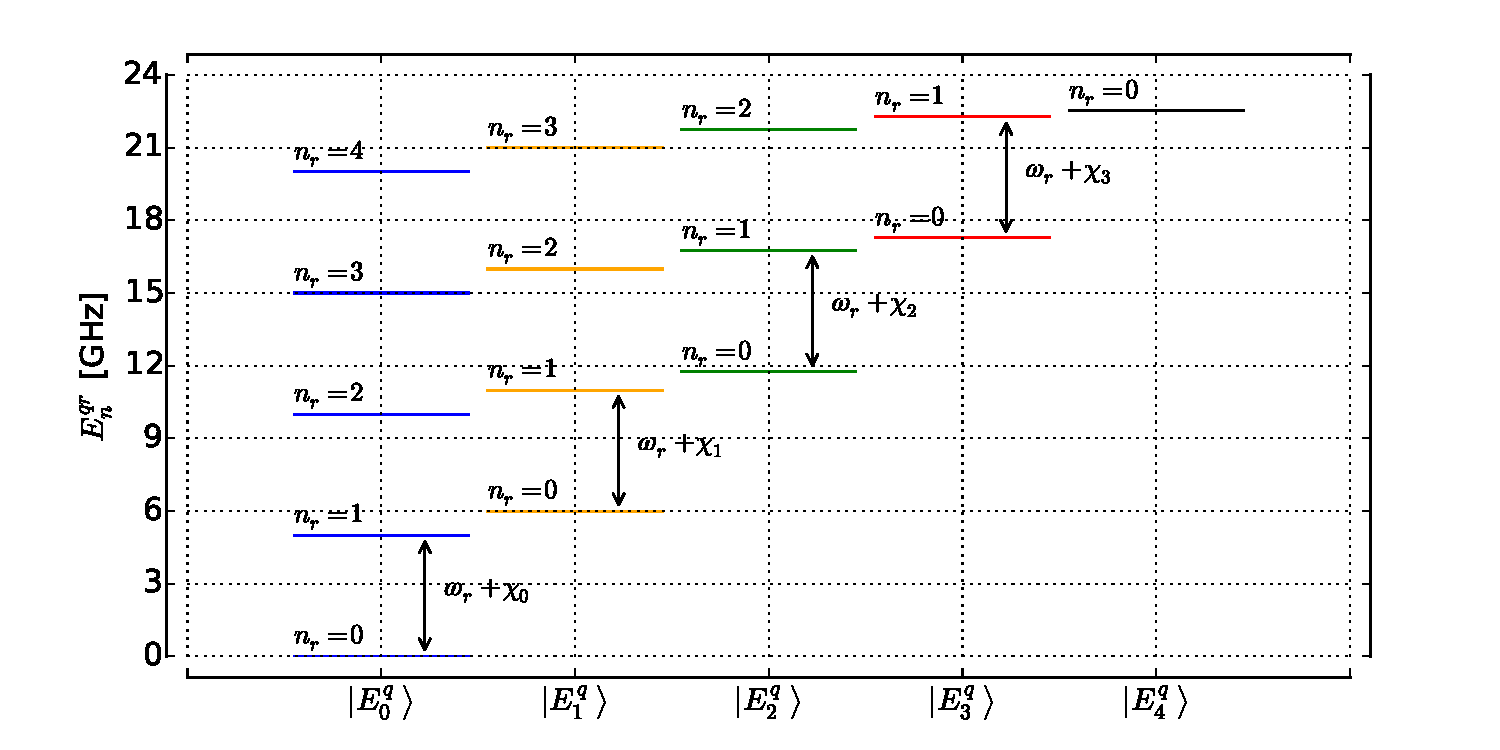
\includegraphics[width=\textwidth]{diagram}
\caption{Energy level diagram for the transmon-resonator system in the sweet spot.}
\label{fig:diagram}
\end{figure}


\section{Energy spectrum of the compound system}

Using QuTiP\cite{Johansson2011} it is straightforward to solve the truncated matrix eigenproblem with the Hamiltonian \eqref{eq:hamiltonian}. The results for the typical design values
$$
C_\kappa = 5 \text{ fF},\ C_g = 2 \text{ fF},\ C_q = 90 \text{ fF},\ C_r = 500 \text{ fF},\ L_r = 20 \text{ nH}, $$
$$E_{J, \Sigma} = (h \nu_q + E_C)^2/8 E_C\ \text{for\cite{Koch2007}}\ \nu_q = 6\ \text{GHz}
$$
can be observed in \autoref{fig:levels}.

In \autoref{fig:diagram} the energy structure of the compound system in the sweet-spot ($\Phi_{ext}=0$) is shown. The dispersively shifted frequencies can be calculated from perturbation theory. For example, for the transition $\ket{0, g}\rightarrow \ket{1, g}$ the shift is defined to the second order as
\begin{align*}
\chi_0 &=  E_{1g}^{(1)} + E_{1g}^{(2)} - E_{0g}^{(1)} - E_{0g}^{(2)}\\
 &= \bra{1, g}\mathcal{\hat H}_i\ket{1,g} + \sum_{i, \alpha \neq 1, g} \frac{|\bra{g, 1}\mathcal{\hat H}_i\ket{i,\alpha} |^2}{E_{1g} - E_{i\alpha}}\\
 & - \bra{0, g}\mathcal{\hat H}_i\ket{0,g} - \sum_{i, \alpha \neq 0, g} \frac{|\bra{g, 0}\mathcal{\hat H}_i\ket{i,\alpha} |^2}{E_{1g} - E_{i\alpha}}.
\end{align*}
As long as $\mathcal{\hat H}_i$ mixes only adjacent resonator states the first order corrections vanish and so do the summations over $i$: $\sum_{i, \alpha} \rightarrow \sum_{0,\alpha} + \sum_{2,\alpha} (\sum_{1,\alpha})$. These sums then can be further truncated:
\begin{equation}
E_{1g}^{(2)} - E_{0g}^{(2)} \approx \frac{|\bra{g,1}\mathcal{\hat H}_i\ket{0,e}|^2}{\omega_r - \omega_{ge}} + \frac{|\bra{g,1}\mathcal{\hat H}_i\ket{2,e}|^2}{\omega_r - 2\omega_r - \omega_{ge}} -
\frac{|\bra{g,0}\mathcal{\hat H}_i\ket{1,e}|^2}{-\omega_r - \omega_{ge}}\label{eq:chi0_truncsums}
\end{equation} 
due to the selection rule of $\hat n$: $\bra{E^q_n}\hat n \ket{E^q_{n+2k}} = 0,\ k \in \mathbb{Z}$ and the fast (exponential from numerics) decay of its matrix elements over distance between transmon energy eigenstates. It can be easily proven that last two elements of \eqref{eq:chi0_truncsums} are equal up to the factor of $\sqrt{2}^2$ and final equation for $\chi_0$ follows
\begin{equation}
\chi_0 = g^2\sbrkt{\frac{n_{ge}^2}{\omega_r - \omega_{ge}}-\frac{n_{ge}^2}{\omega_r + \omega_{ge}}}.
\end{equation}
Similarly, dispersive shifts for the other two transmon states are derived:
\begin{gather*}
\chi_1 = g^2\sbrkt{\frac{n_{ef}^2}{\omega_r - \omega_{ef}} - \frac{n_{ef}^2}{\omega_r + \omega_{ef}} + \frac{n_{eg}^2}{\omega_r + \omega_{ge}}+ \frac{n_{eg}^2}{\omega_{ge}-\omega_r }},\\
\chi_2 = g^2\sbrkt{\frac{n_{fd}^2}{\omega_r - \omega_{fd}} -\frac{n_{fd}^2}{\omega_r + \omega_{fd}} + \frac{n_{fe}^2}{\omega_r + \omega_{ef}}+ \frac{n_{fe}^2}{\omega_{ef}-\omega_r}},
\end{gather*}
where $g, e, f, d$ denote the first 4 energy eigenstates of the transmon, $n_{\alpha\beta} = \bra{\alpha} \hat n \ket{\beta}$ is the matrix element of $\hat n$ and $g = \left.|\frac{\mathcal{\hat H}_i}{i(\hat a^\dag  - \hat a)\otimes \hat n}|\right.$ is the coupling parameter which precedes the operator part in the interaction Hamiltonian. These formulas were compared to the numerical solution and have relative errors of less than 1\%.
\chapter{Dynamics}

\section{Driving of an isolated transmon (Xmon)}

To simulate the dynamics in the unitary case without taking into account the dissipative processes it is enough to solve Schrödinger equation with the Hamiltonian \eqref{eq:hamiltonian} summed with the driving part \eqref{eq:driving_q}. To consider the isolated qubit only it is sufficient to put $C_g = 0$. The final state after some time of the evolution $t$ will be described with a Dyson series or a $\hat T$-exponent:
\begin{equation}
\ket{\psi}(t) = \hat T \exp\left\{-\frac{i}{\hbar} \rbrkt{\mathcal{\hat H}t + \int_0^t \mathcal{\hat H}_q^d(\tau) \diff\tau}\right\} \ket{E_0^q}= \sum_k c_k(t) \ket{E^q_k},
\end{equation} 
where $\ket{E_k^q}$ denotes the $k$'s eigenstate of the qubit Hamiltonian. The simulation can also be reduced to a standard linear ODE solution which is also possible within QuTiP framework using the \textit{mesolve} routine.

The result of such simulation can be observed in \autoref{fig:driven_tr}. As one can see when the driving amplitude (in GHz) becomes comparable to the anharmonicity of the transmon significant leakage to higher states occurs.

\begin{figure}[h!]
\centering
\begin{subfigure}[t]{0.45\textwidth}
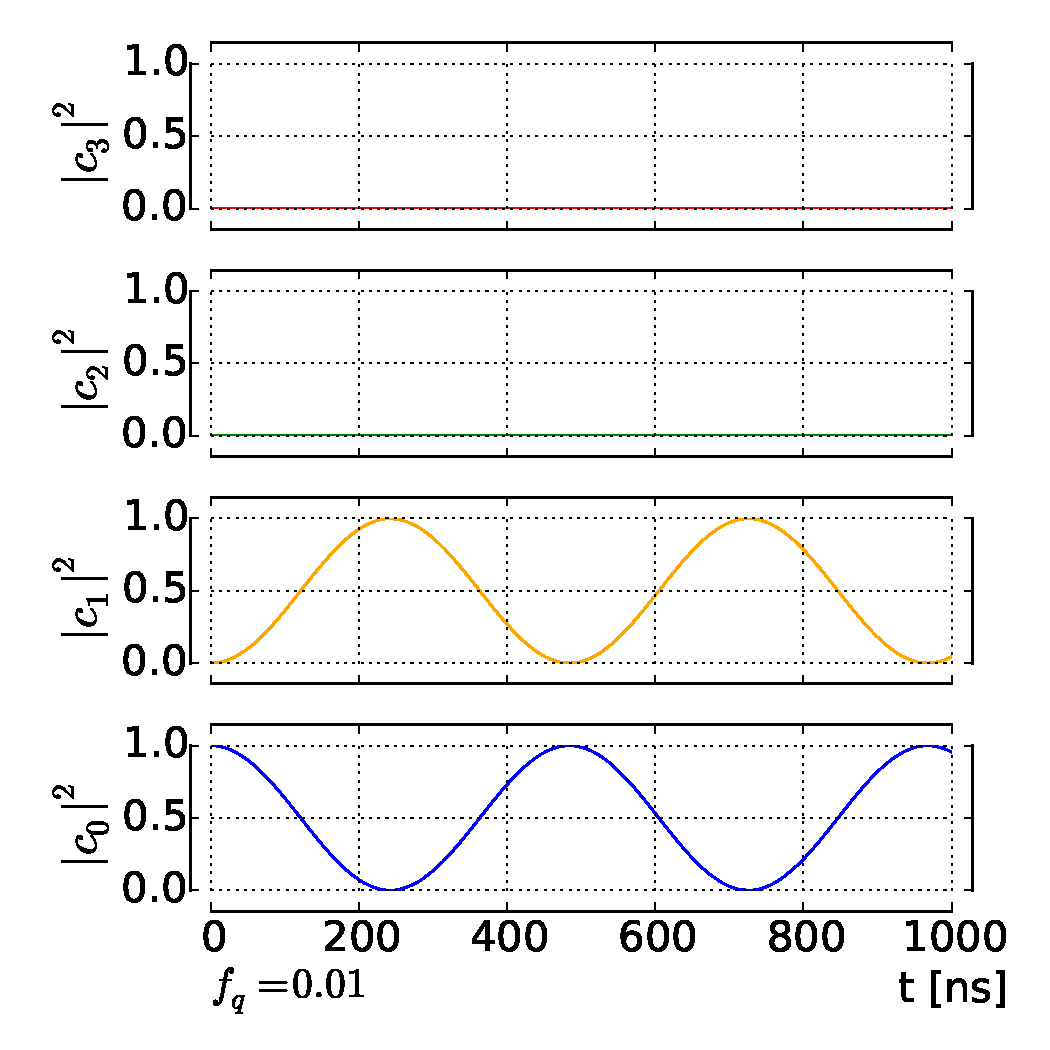
\includegraphics[width=\textwidth]{tr_weak_dr}
\end{subfigure}
\begin{subfigure}[t]{0.45\textwidth}
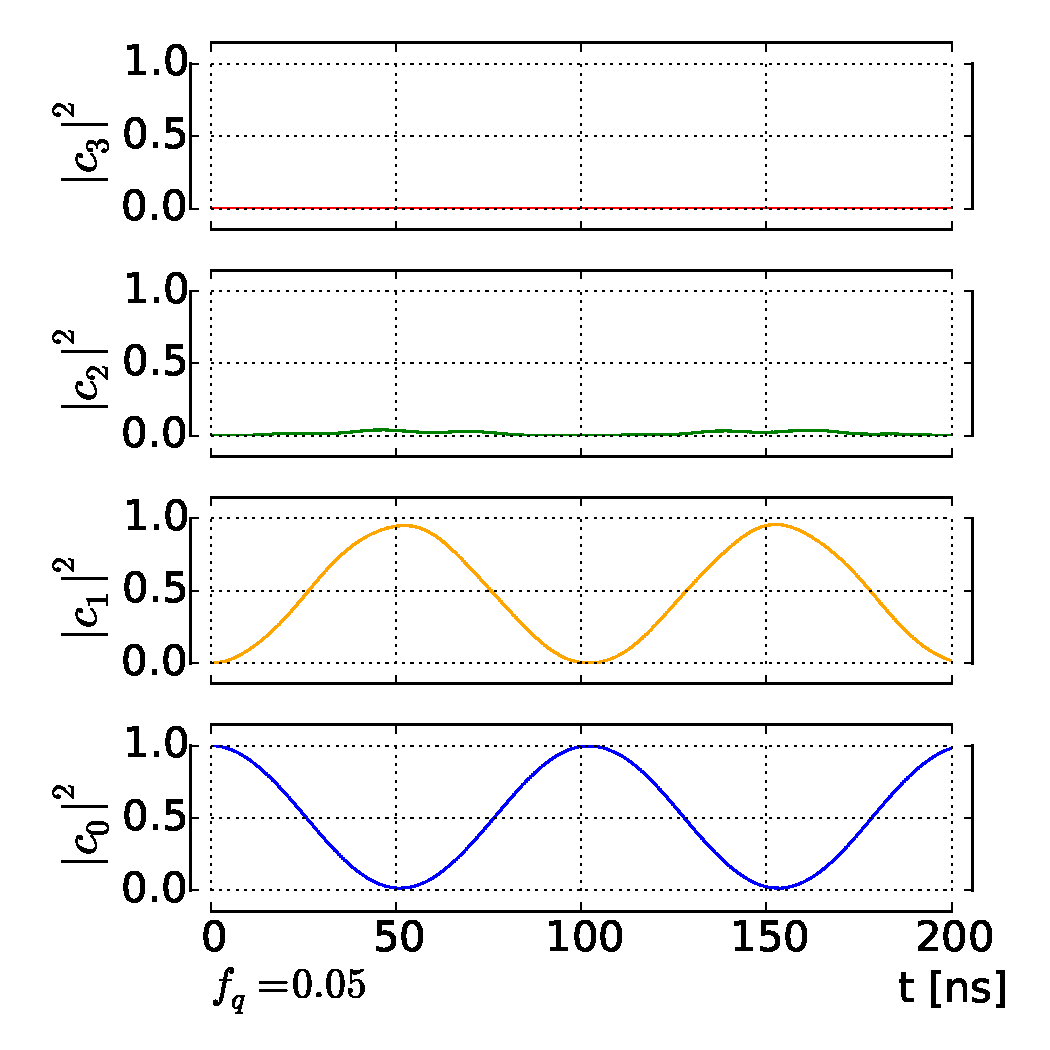
\includegraphics[width=\textwidth]{tr_int_dr}
\end{subfigure}

\begin{subfigure}[t]{0.45\textwidth}
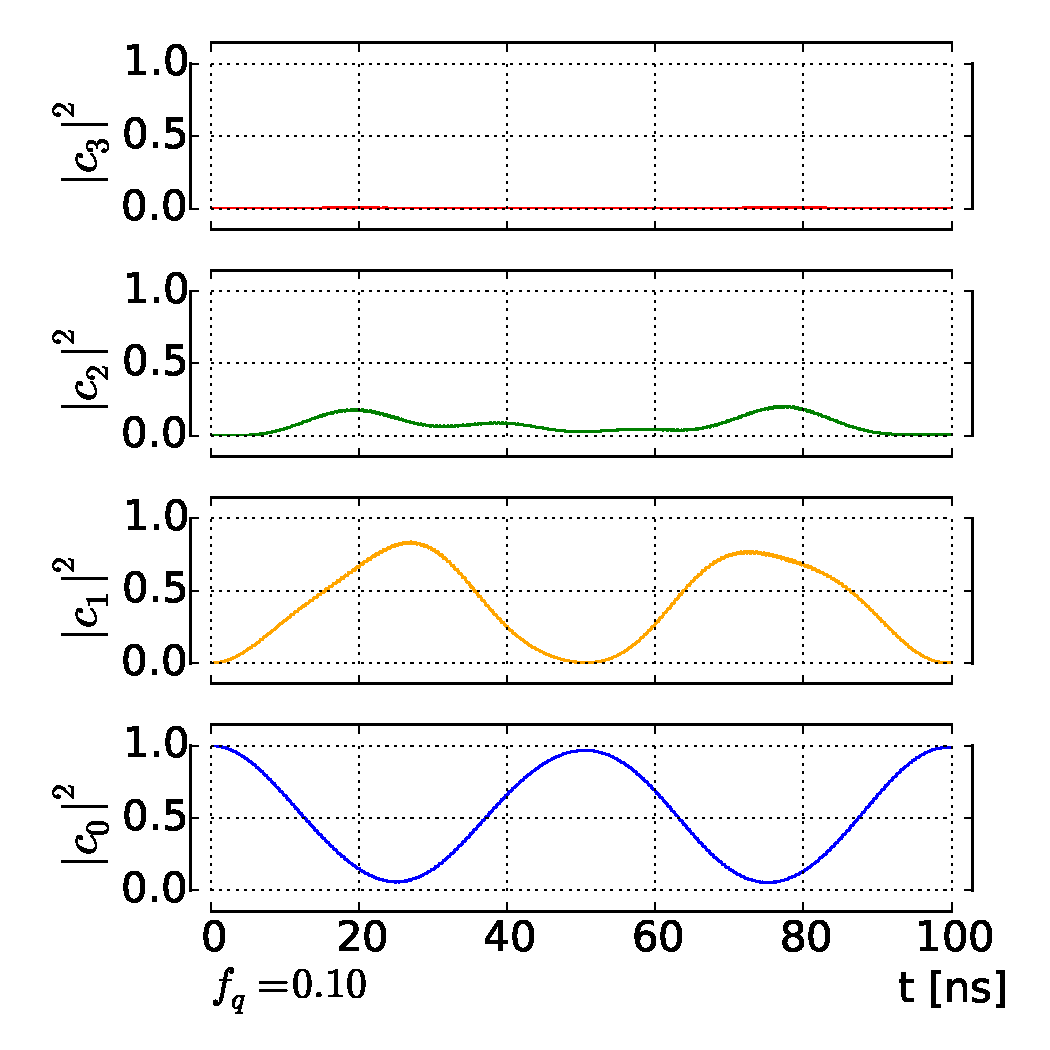
\includegraphics[width=\textwidth]{tr_str_dr}
\end{subfigure}
\begin{subfigure}[t]{0.45\textwidth}
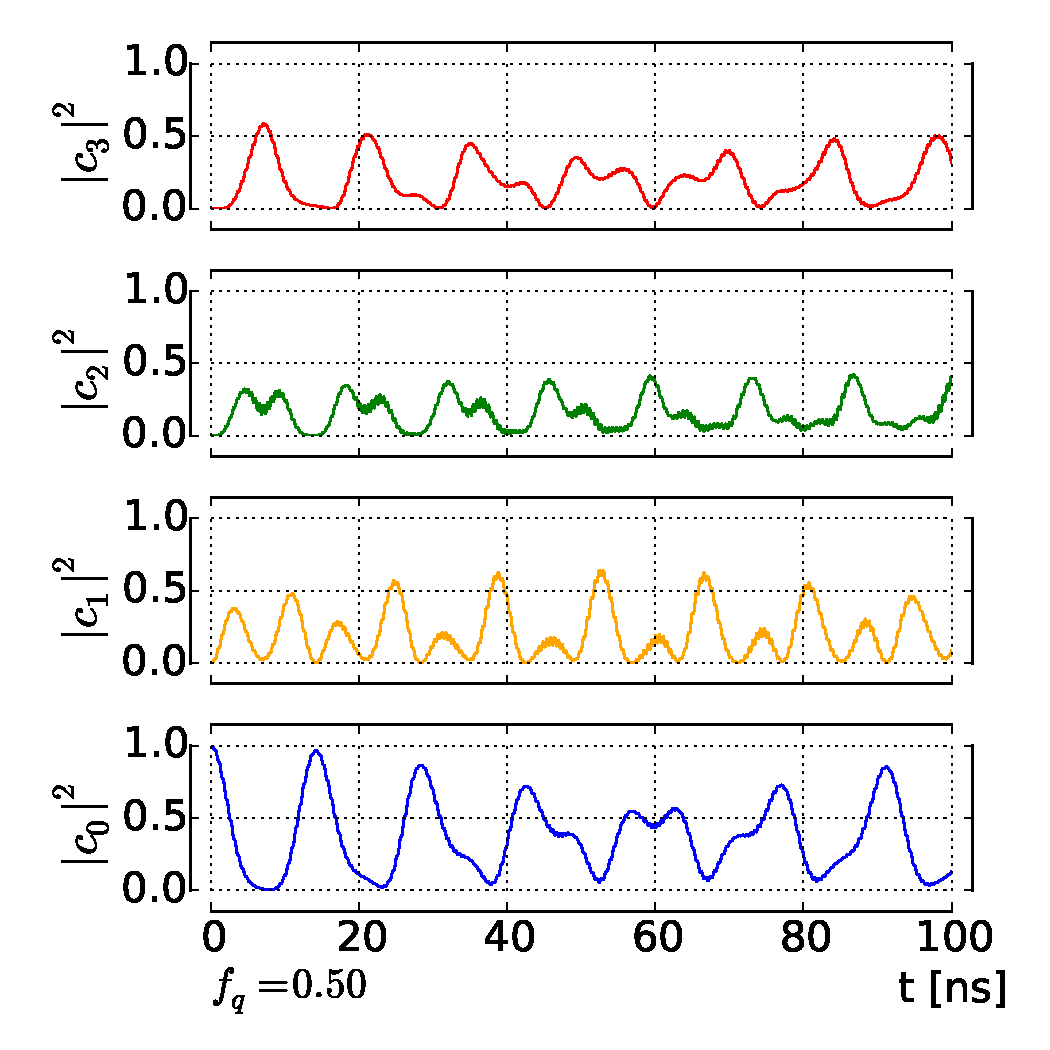
\includegraphics[width=\textwidth]{tr_vstr_dr}
\end{subfigure}
\caption{Dynamics of the isolated driven transmon qubit with different drive strengths $f_q$ = 0.01-0.5 GHz, where $f_q$ is an effective amplitude of the drive \eqref{eq:driving_q} $f_q (t) = f_q \sin(\omega_{01} t)$. It can be seen that significant distortions and leakage to higher levels occur when amplitude is too large.}
\label{fig:driven_tr}
\end{figure}

\appendix

\chapter{Pure dephasing or Does the density matrix really exist?}

There are two ways of describing pure dephasing. One is developed from the system-bath approach (Lindbladian master equation) and the other comes from the stochastic Schrödinger equation. However the results of the latter deviate fundamentally from the results of the former for the experiment of spin-echo for a single qubit. Here this problem will be described in detail.

\section{Quantum derivation of dephasing}

For the derivation of this phase-destroying process in a quantum way the system-bath interaction Hamiltonian part is chosen as
\[
\mathcal{\hat H}_{sb} = \hat \sigma_z \otimes \hat O_b, 
\]
where $\hat O_b$ is an arbitrary bath operator. From this interaction term a master equation is then developed:
\[
\partial_t \hat \rho_s = \frac{i}{\hbar}[\hat \rho_s, \mathcal{\hat H}_s] + \gamma_\phi (\hat \sigma_z \hat \rho_s \hat \sigma_z - \hat \rho_s).
\]
The dynamics of this equation can be seen in \autoref{fig:qdeph}.  At $t \rightarrow \infty$ the state of the system is a totally mixed state:
\[
\hat \rho_s (\infty) = \rbrkt{\begin{matrix}
0.5 & 0 \\
0 & 0.5 
\end{matrix}}.
\]
Following the open system approach this should be understood as the consequence of the entanglement of the qubit with the environment. The same density matrix we will obtain trying to find out in which state
is the qubit $A$ when it's a part of a composite system $A \otimes B$ of two qubits being in a Bell  state $\ket{\Psi^+} = \frac{1}{\sqrt{2}}(\ket{0}_A\otimes\ket{1}_B+\ket{1}_A\otimes\ket{0}_B)$. From the quantum point of view therefore the process of dephasing is irreversible.
\begin{figure}
\centering
\begin{subfigure}[t]{0.45\textwidth}
\centering
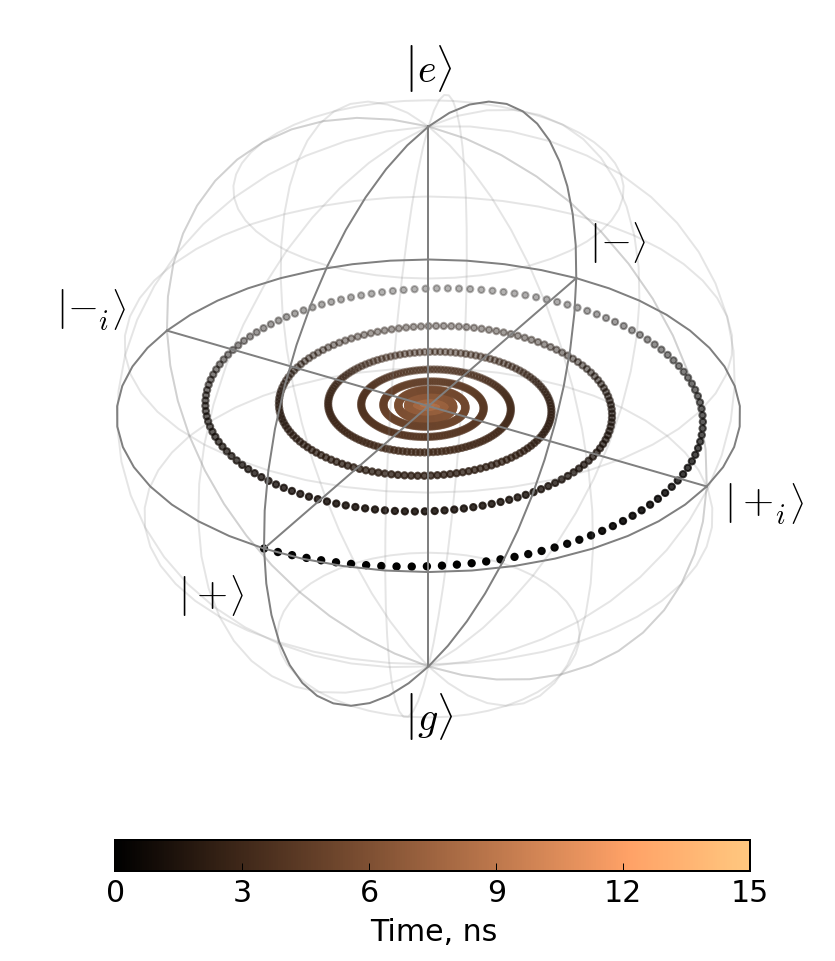
\includegraphics[width=0.9\textwidth]{qdeph_bloch}
\caption{Dephasing on the Bloch sphere.}
\end{subfigure}
\begin{subfigure}[t]{0.45\textwidth}
\centering
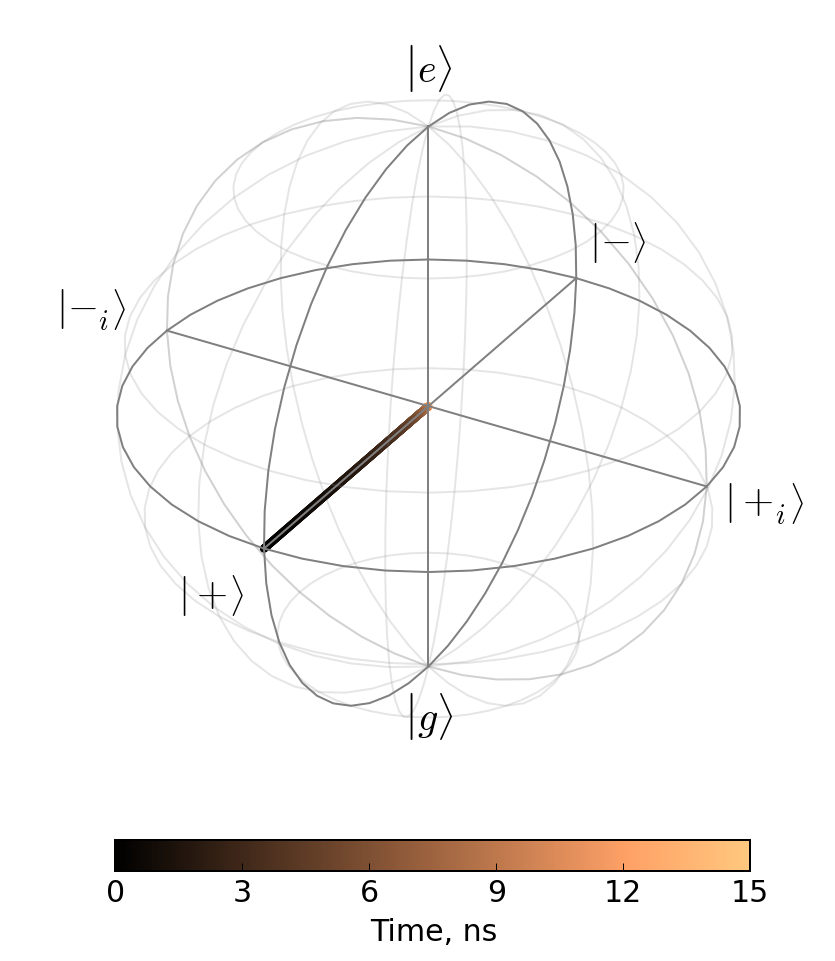
\includegraphics[width=0.9\textwidth]{qdeph_bloch_rf}
\caption{Same within the rotating frame.}
\end{subfigure}

\begin{subfigure}[t]{0.45\textwidth}
\centering
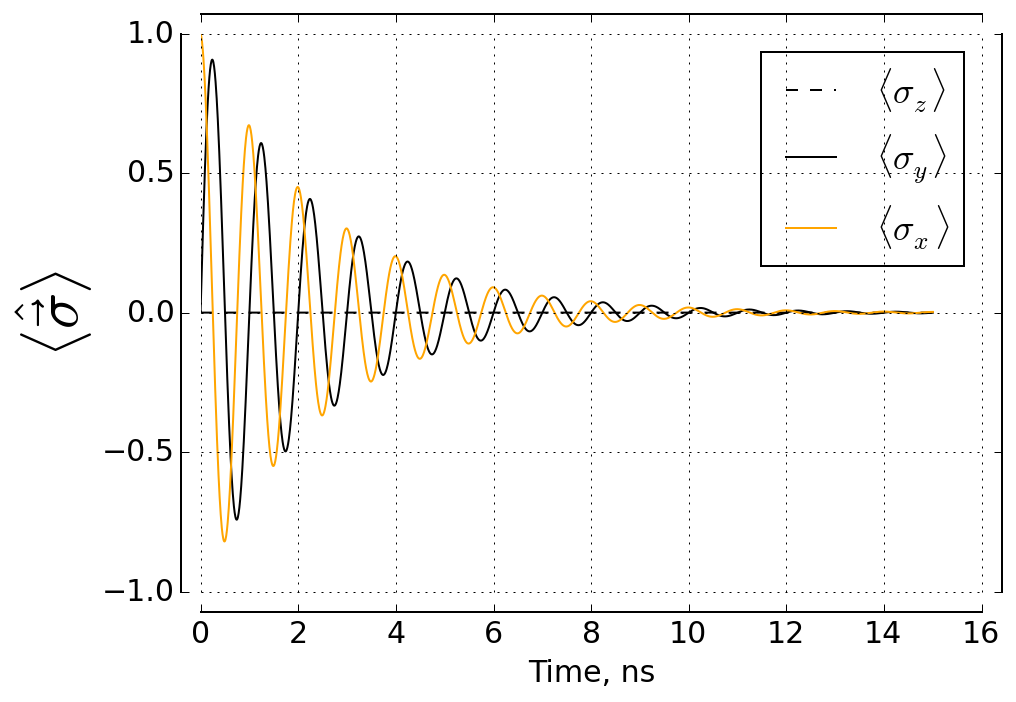
\includegraphics[width=0.9\textwidth]{qdeph_xyz}
\caption{Decay of the $\langle \hat \sigma_{x, y} \rangle$ components.}
\end{subfigure}
\begin{subfigure}[t]{0.45\textwidth}
\centering
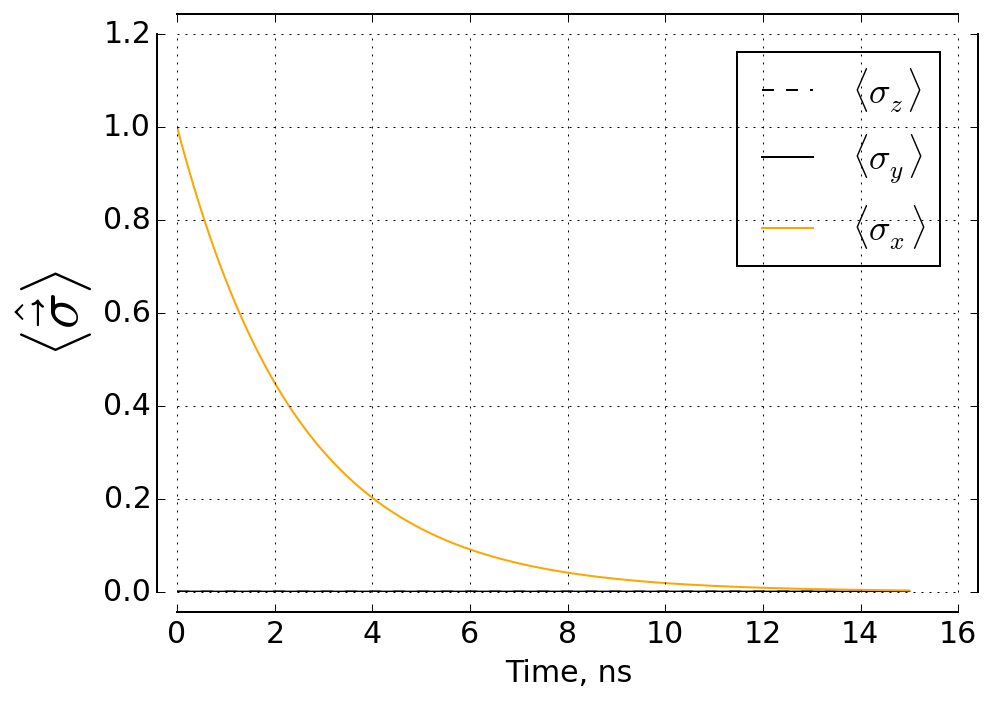
\includegraphics[width=0.9\textwidth]{qdeph_xyz_rf}
\caption{Same within the rotating frame.}
\end{subfigure}
\caption{Dephasing treated quantum-mechanically shows exponential decrease of the coherences of the density matrix.}
\label{fig:qdeph}
\end{figure}

\section{Classical derivation of dephasing}

The classical derivation will be presented below in detail. This method, just as in the case of interaction of an atom with a classical field, just includes an additional time-dependent term in the Hamiltonian, representing fluctuations of the system's parameters. For the pure dephasing this term looks like $f(t) \hat \sigma_z$, where $f(t)$ is the random noise. It is possible to write down the evolution of the density matrix for such noisy Schrödinger equation. Until specified, the unitary evolution will be discussed, although using density matrix. In the rotating frame:
\[
\hat \rho_s (t) = \hat U^\dag(t, 0)\ \hat\rho\ \hat U(t, 0), 
\]
where 
\[
U(t, 0) = \hat T \exp \left\{-\frac{i}{\hbar} \int_0^t f(\tau)\hat \sigma_z \diff\tau\right\}.
\]
From the fact that $\hat \sigma_z$ is diagonal it can be shown that
\[
\begin{gathered}
\hat \rho_s (t) = \rbrkt{\begin{matrix}
\exp \left\{\frac{i}{\hbar} \int_0^t f(\tau_1) \diff\tau_1\right\} & 0\\
0 & \exp \left\{-\frac{i}{\hbar} \int_0^t f(\tau_1) \diff\tau_1\right\}
\end{matrix}}\cdot\\
\cdot\rbrkt{\begin{matrix}
1/2 - N(0)/2 & \rho(0) \\
\rho^*(0) & 1/2 + N(0)/2 
\end{matrix}}\cdot\\
\cdot\rbrkt{\begin{matrix}
\exp \left\{-\frac{i}{\hbar} \int_0^t f(\tau_2)\diff\tau_2\right\} & 0\\
0 & \exp \left\{+\frac{i}{\hbar} \int_0^t f(\tau_2)\diff\tau_2\right\}
\end{matrix}},
\end{gathered}
\] 
where the integral variables $\tau_1$ and $\tau_2$, coherence $\rho(t)$ and inversion $N(t)$ where introduced. From above it is obvious that
\begin{gather}
N(t) = N(0)\\
\rho(t) = \rho(0)\exp \left\{ \frac{2i}{\hbar}\int_0^t f(\tau)  \diff \tau \right\}. \label{eq:rho_t}
\end{gather}
This equations can be visualized with numerical simulation, taking $f(t)$ be, for instance, normally distributed. Phase will experience random drifts, which lead to random rotations of the Bloch vector on the equator of the sphere, see \autoref{fig:cdeph}~(a), (c).

However, we can now use the other side of the density matrix, the property for which it is also called statistical operator. Let's run the equation \eqref{eq:rho_t} many times and look at the statistically expected state of the observed system over time. The diagonal part will still stay the same, and for coherence we have (presuming Gaussian instantaneous distribution of $f(t)$ and $x(t) = \frac{2}{\hbar}\int_0^t f(\tau)  \diff \tau$):
\begin{gather}
\langle \rho(t) \rangle = \rho(0) \int_{-\infty}^{+\infty} e^{ix}\, \mathbb{N}_{0,\sigma}(x) \diff x = \rho(0) e^{-\sigma^2/2} = \rho(0) e^{-\langle x^2 \rangle/2} \\
= \rho(0)\exp \left\{ -\frac{2}{\hbar^2}\int_0^t\int_0^t \langle f(\tau_1) f(\tau_2) \rangle \diff \tau_1 \diff \tau_2 \right\}.
\end{gather}
Presuming also that $f(t)$ is a wide-sense stationary process $\langle f(\tau_1) f(\tau_2) \rangle = K(\tau_2 - \tau_1) = \frac{1}{\sqrt{2\pi}}\int\limits_\mathbb{R} S(\omega) e^{i\omega(\tau_2-\tau_1)}\diff\omega$ where $S(\omega)$ is the power spectral density of $f(t)$. Taking the time integrals with the exponents, finally we obtain
\begin{equation}
\langle \rho(t) \rangle = \rho(0) \exp  \left\{-\frac{2}{\sqrt{2\pi}\hbar^2} \int\limits_\mathbb{R} \frac{4 \sin^2(\frac{\omega t}{2})}{\omega^2} S(\omega)\diff \omega \right\}.\label{eq:cdeph}
\end{equation}
It can be shown easily that \eqref{eq:cdeph} is an exponent for either a white noise ($S(\omega) = S(0) = const$) or for a sufficiently large time $t$ where 
$$\frac{t}{2}\int\limits_\mathbb{R} \diff(\omega t/2) \frac{\sin^2(\frac{\omega t}{2})}{(\omega t/2)^2} \ \bullet $$
acts as $ \frac{t\pi}{2}\delta(\omega)\ \bullet$. In both this cases pure dephasing rate $\Gamma^*_2$ exists in a usual sense and $\Gamma^*_2 \propto S(0)$. In case of, for example, 1/f noise the decay curve will have the shape of $e^{-t^2}$ in the vicinity of $t=0$.

The averaged evolution for the white noise case can be observed in \autoref{fig:cdeph}~(b), (d). It is very similar to what can be seen in \autoref{fig:qdeph}. 1000 trajectories were used for averaging.
In \autoref{fig:cdeph_pink} the simulation of the dynamics under the 1/f noise is shown. For the averaged case ((b), (d)) 2500 trajectories where used. One can see that a plateau is present for the yellow graph near $t=0$, in accordance with theoretical predictions.
\begin{figure}
\begingroup
\captionsetup[subfigure]{width=0.9\textwidth}
\centering
\begin{subfigure}[t]{0.45\textwidth}
\centering
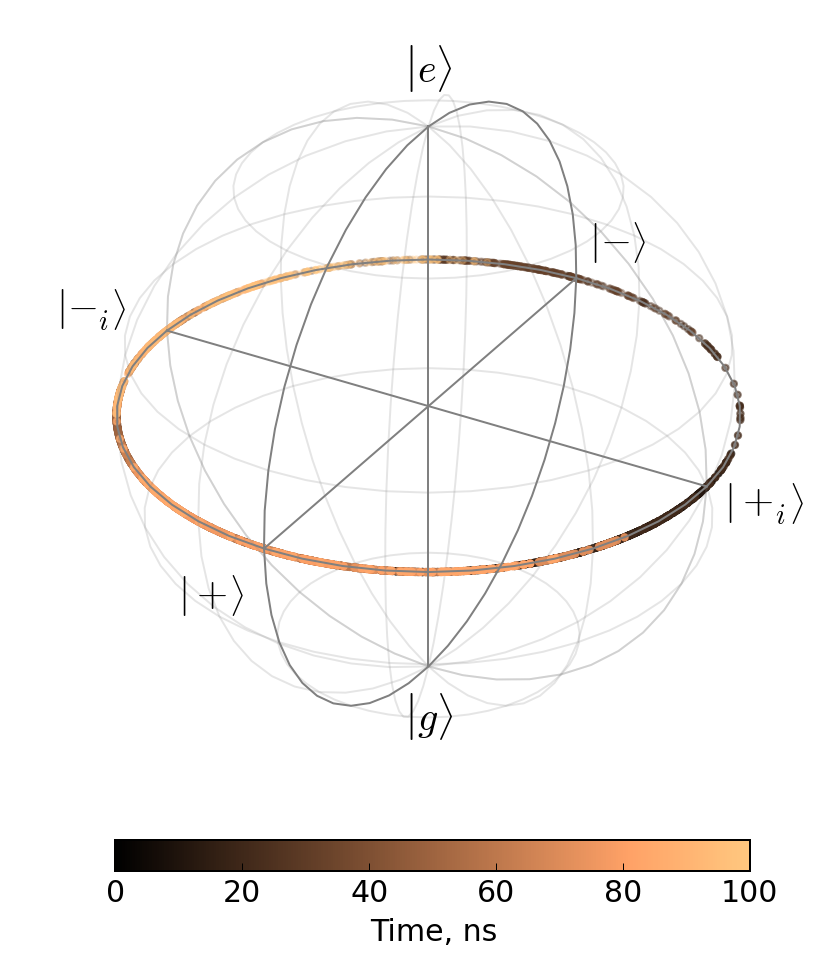
\includegraphics[width=0.9\textwidth]{cdeph_bloch_rf}
\caption{White Gaussian noise affecting the phase in the rotating frame.}
\end{subfigure}
\begin{subfigure}[t]{0.45\textwidth}
\centering
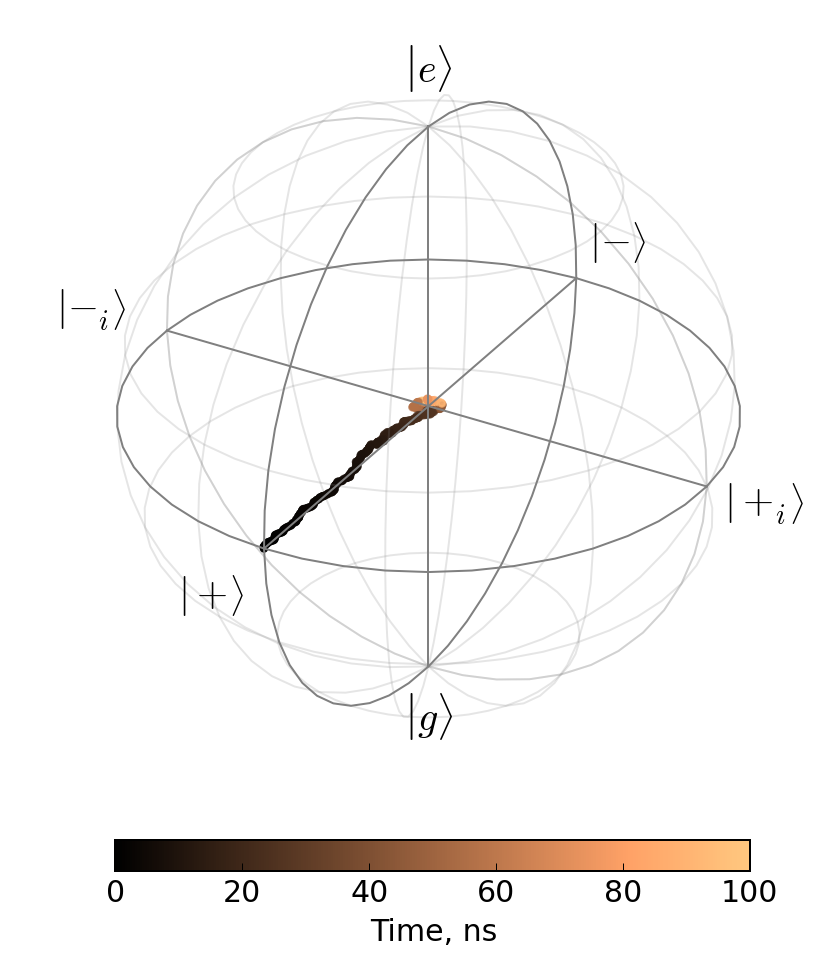
\includegraphics[width=0.9\textwidth]{cdeph_bloch_rf_avg}
\caption{Averaged dynamics in the rotating frame.}
\end{subfigure}

\begin{subfigure}[t]{0.45\textwidth}
\centering
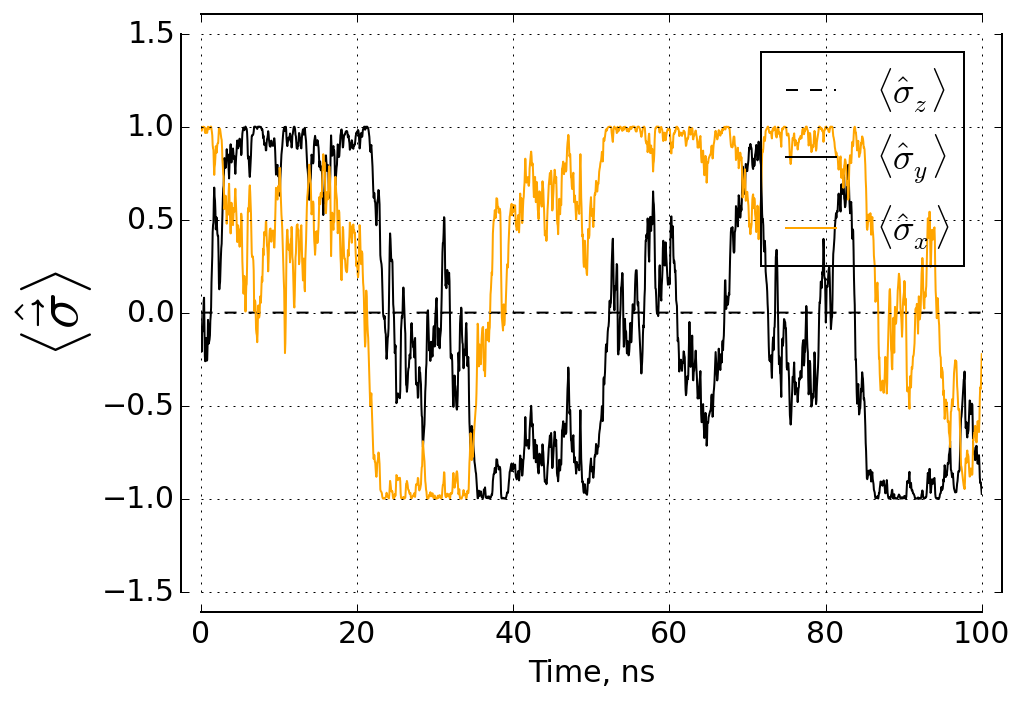
\includegraphics[width=0.9\textwidth]{cdeph_xyz_rf}
\caption{Behaviour of the $xyz$ components in the rotating frame.}
\end{subfigure}
\begin{subfigure}[t]{0.45\textwidth}
\centering
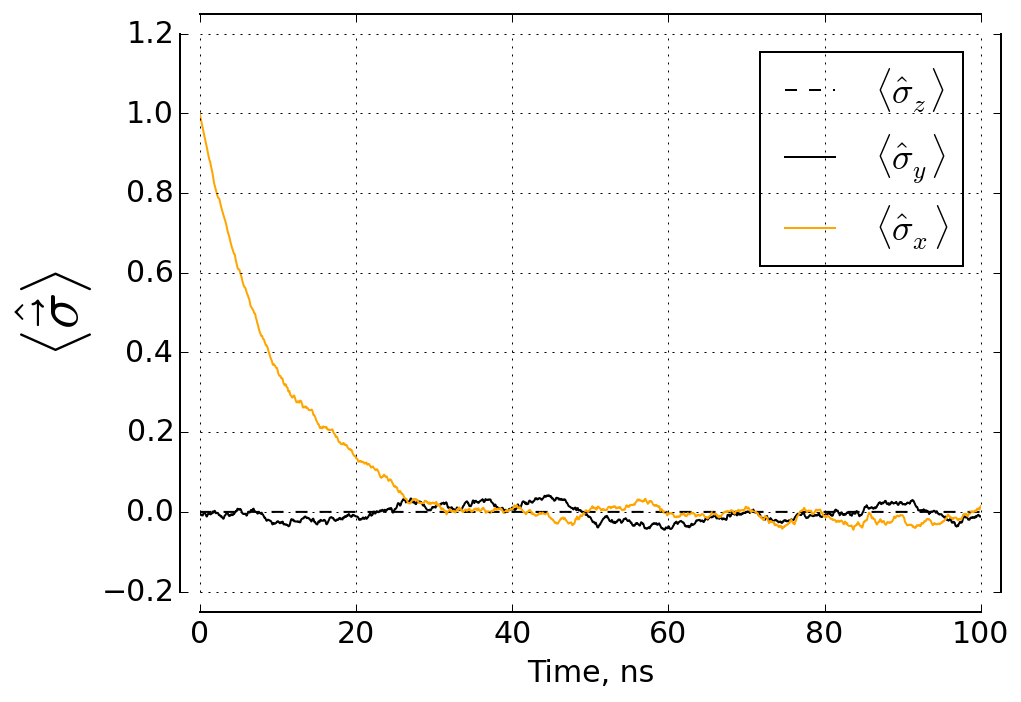
\includegraphics[width=0.9\textwidth]{cdeph_xyz_rf_avg}
\caption{Averaged behaviour of the $xyz$ components in the rotating frame.}
\end{subfigure}
\caption{Classically treated pure dephasing for white noise.}
\label{fig:cdeph}
\endgroup
\end{figure}

\begin{figure}
\begingroup
\captionsetup[subfigure]{width=0.9\textwidth}
\centering
\begin{subfigure}[t]{0.45\textwidth}
\centering
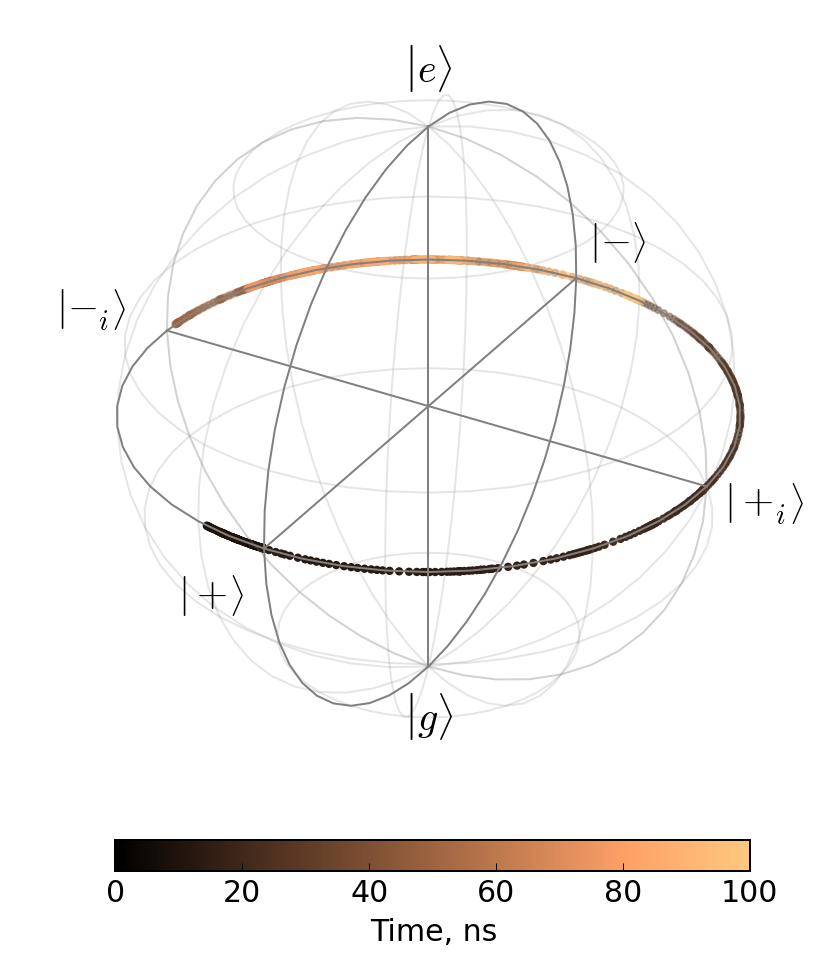
\includegraphics[width=0.9\textwidth]{cdeph_bloch_rf_pink}
\caption{1/f Gaussian noise affecting the phase in the rotating frame.}
\end{subfigure}
\begin{subfigure}[t]{0.45\textwidth}
\centering
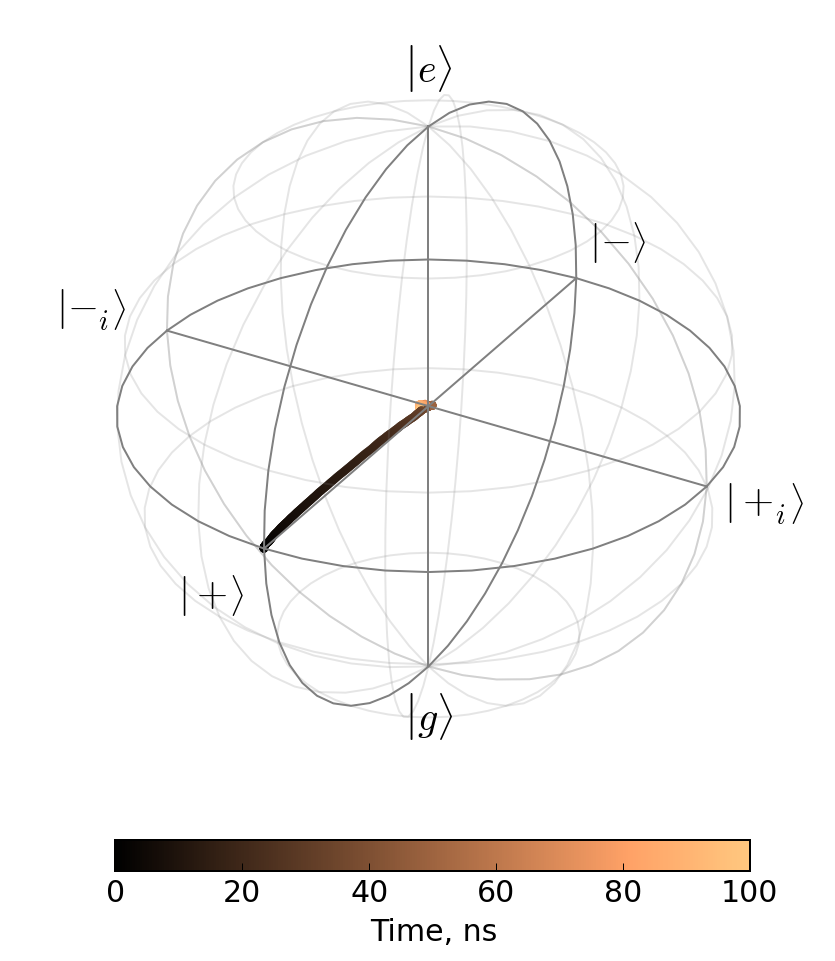
\includegraphics[width=0.9\textwidth]{cdeph_bloch_rf_avg_pink}
\caption{Averaged dynamics in the rotating frame.}
\end{subfigure}

\begin{subfigure}[t]{0.45\textwidth}
\centering
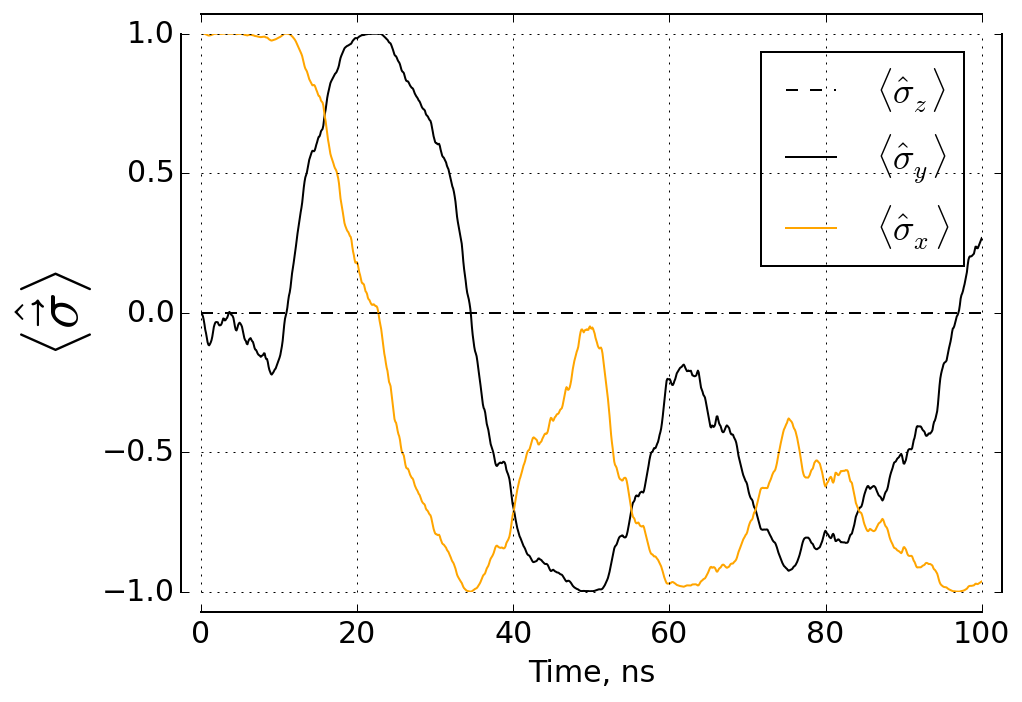
\includegraphics[width=0.9\textwidth]{cdeph_xyz_rf_pink}
\caption{Behaviour of the $xyz$ components in the rotating frame.}
\end{subfigure}
\begin{subfigure}[t]{0.45\textwidth}
\centering
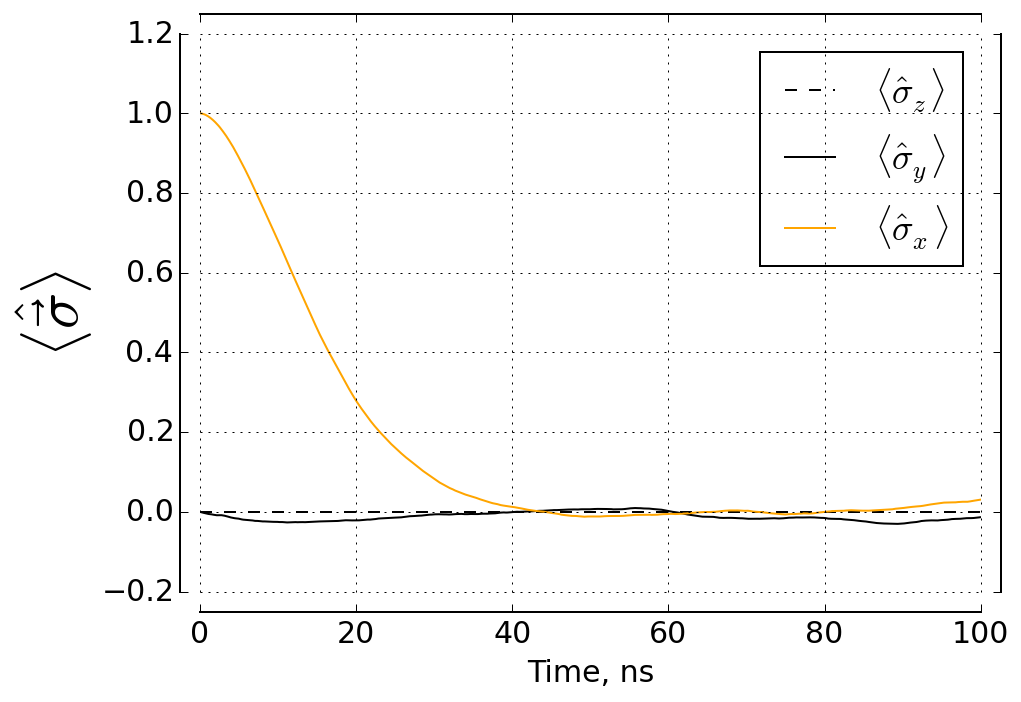
\includegraphics[width=0.9\textwidth]{cdeph_xyz_rf_avg_pink}
\caption{Averaged behaviour of the $xyz$ components in the rotating frame.}
\end{subfigure}
\caption{Classically treated pure dephasing for 1/f noise.}
\label{fig:cdeph_pink}
\endgroup
\end{figure}

\section{Spin-echo experiment}

The spin-echo experiment in the simplest case (Hahn echo) is a modification of a Ramsey pulse sequence with an additional $\pi_y$-pulse right in between the $\frac{\pi}{2}_x$ ones. The idea is that during the second period (after the $\pi_y$-pulse)  slow components of the noise will cancel out the phase difference they've imposed during the first period. This can be understood easily in the limit of constant noise and infinitely fast rotations. There are also more sophisticated echo sequences such as CP, CPMG and UDD\cite{Bylander2011} which use more than one $\pi_y$-pulse during the free evolution, however for our case it is enough to regard the simplest Hahn echo.

Mathematically Hahn echo within the previous formulations acts as follows. Before the  $\pi_y$-pulse at time $t/2$ we have the same dynamics described by the \eqref{eq:rho_t}. Than instantaneously the coherences of the density matrix are complex conjugated as a result of an infinitely fast $\pi_y$-pulse. This can be understood from the result of $\pi_y$-pulse on the Bloch sphere: $\left< \hat \sigma_x \right> = \rho + \rho^* \overset{\pi_y}{\rightarrow}  \left< \hat \sigma_x \right>,\ \left< \hat \sigma_y \right> = i(\rho - \rho^*) \overset{\pi_y}{\rightarrow} -\left< \hat \sigma_y \right>,\ \left< \hat \sigma_z \right> = N  \overset{\pi_y}{\rightarrow}  \left< \hat \sigma_z \right>$. Finally, for the changed initial condition at $t/2$ again evolution \eqref{eq:rho_t} is applied. Therefore, at the end of the period the coherence is defined as
\begin{equation*}
\rho(t) = \rho(0)\exp \left\{ - \frac{2i}{\hbar}\int_0^{t/2} f(\tau)  \diff \tau + \frac{2i}{\hbar}\int_{t/2}^{t} f(\tau)  \diff \tau \right\}.
\end{equation*}
Performing the ensemble averaging one can get
\begin{gather*}
\left<\rho(t)\right> = \rho(0)\exp \left\{ - \frac{2}{\hbar^2} \left< \left( \int_0^{t/2} f(\tau_1)  \diff \tau_1 + \int_{t/2}^{t} f(\tau_2)  \diff \tau_2 \right)\cdot \right. \right. \\
\cdot \left. \left. \left( \int_0^{t/2} f(\tau_3)  \diff \tau_3 + \int_{t/2}^{t} f(\tau_4)  \diff \tau_4 \right) \right> \right\}.
\end{gather*}
Expanding the brackets, again putting a Fourier transform of the power spectral density $S(\omega)$ instead of the autocorrelation functions and factoring the expression back to the initial representation it is possible to obtain\cite{Preskill} the final expression for the coherence expectation:
\begin{equation}
\left<\rho(t)\right> = \rho(0)\exp \left\{ - \frac{2}{\sqrt{2\pi} \hbar^2} \int_\mathbb{R} S(\omega) W_t (\omega) \right\},
\label{eq:cdeph_se}
\end{equation}
where
\begin{align*}
 W_t (\omega)  &= \left| - \int_0^{t/2} e^{i \omega \tau}\diff \tau + \int_{t/2}^{t} e^{i\omega\tau}  \diff \tau  \right|^2 \\
& =  \left| 1-2e^{i\omega t/2} + e^{i\omega t} \right| \\
&= \left| \frac{(1-e^{i\omega t/2})}{(1+e^{i\omega t/2})} (1+e^{i\omega t/2})(1-e^{i\omega t/2})\right|\\
& = \tan^2(\omega t/4)\frac{4 \sin^2(\omega t/2)}{\omega^2}.
\end{align*}
It's obvious from \eqref{eq:cdeph_se}  that the noise influence is now suppressed at low frequencies (compare with \eqref{eq:cdeph}) however it is enhanced at some higher frequency. This leads to inefficiency of Hahn echo and similar techniques when the noise is white and a good $T_2^*$ improvement when it's 1/f, see \autoref{fig:cdeph_both}.


\begin{figure}
\begingroup
\captionsetup[subfigure]{width=0.9\textwidth}
\centering
\begin{subfigure}[t]{0.45\textwidth}
\centering
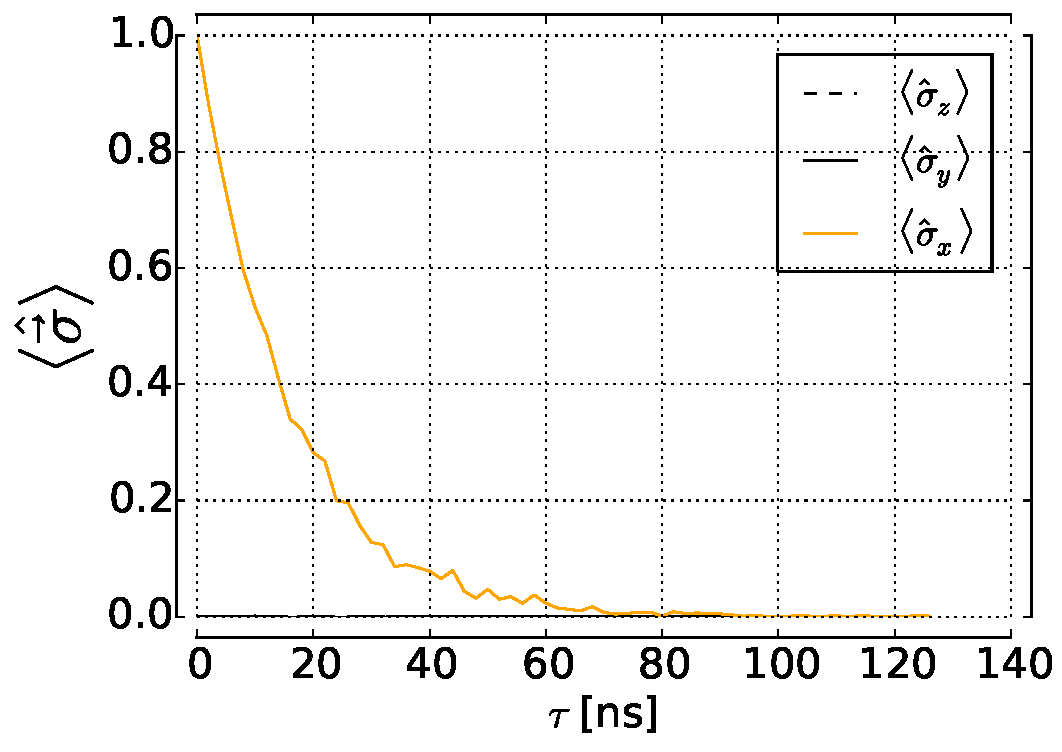
\includegraphics[width=0.9\textwidth]{deph_white}
\end{subfigure}
\begin{subfigure}[t]{0.45\textwidth}
\centering
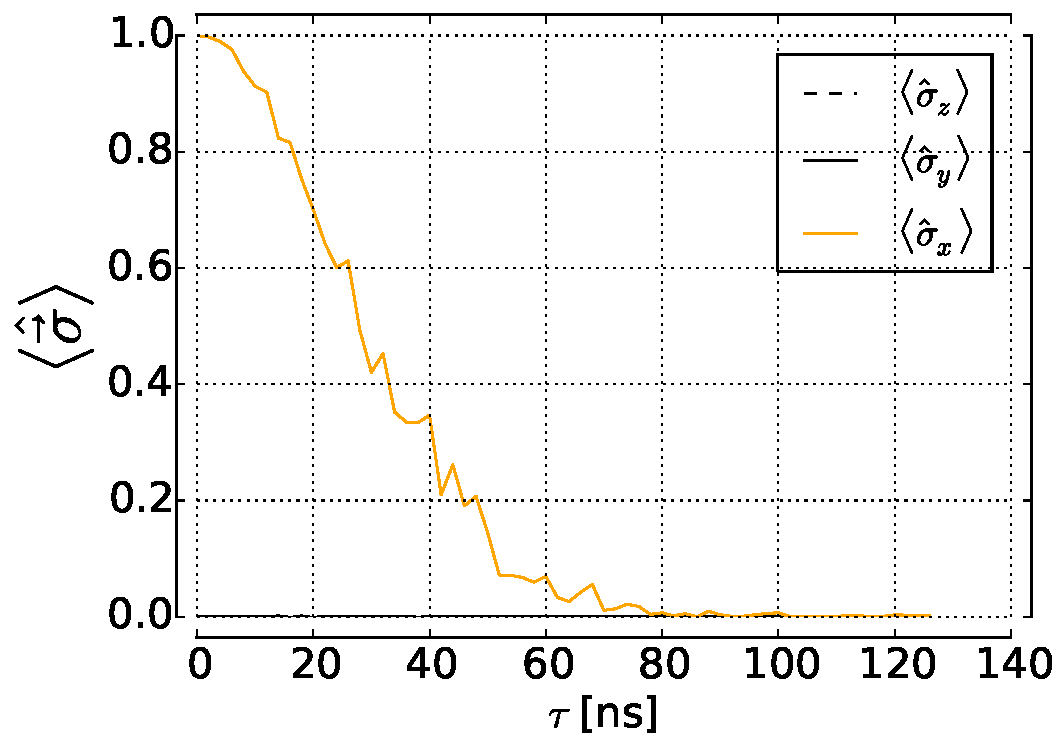
\includegraphics[width=0.9\textwidth]{deph_pink}
\end{subfigure}

\begin{subfigure}[t]{0.45\textwidth}
\centering
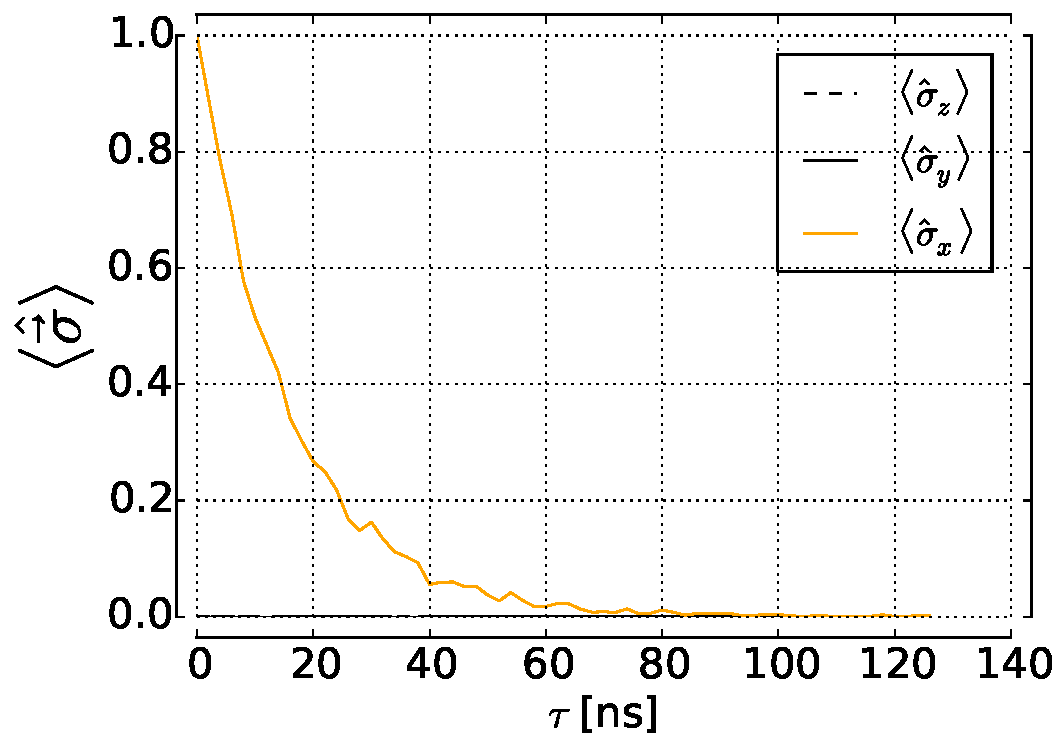
\includegraphics[width=0.9\textwidth]{deph_white_se}
\end{subfigure}
\begin{subfigure}[t]{0.45\textwidth}
\centering
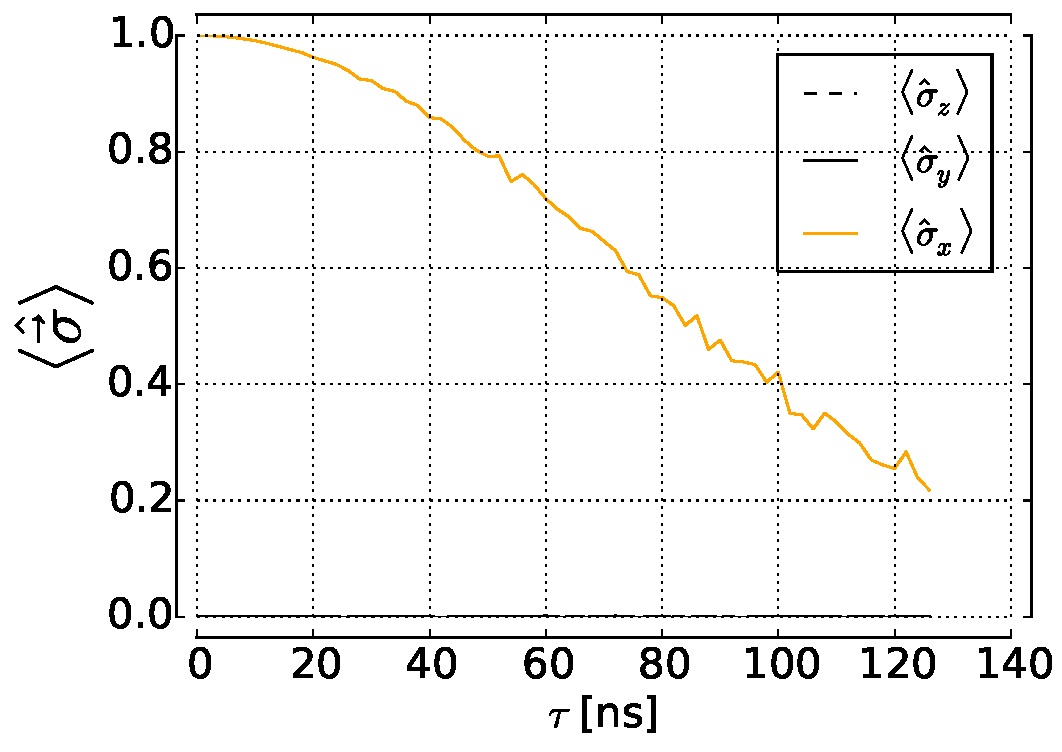
\includegraphics[width=0.9\textwidth]{deph_pink_se}
\end{subfigure}
\caption{Decoherence under white (left) and 1/f (right) noises with (bottom) and without (top) a refocusing $\pi_y$-pulse.}
\label{fig:cdeph_both}
\endgroup
\end{figure}

\section{The problem (of Markovian MEs)}

The interesting correspondence between quantum and classical derivation can be noted within the spin echo experiment. For the white noise both of the descriptions yield same results, the exponential decay of coherences with an equal rate. However the meanings of these two results are completely different. Quantum approach tells us that the density matrix will emerge even in a single experiment as a consequence of entanglement with the environment. Classical approach tells us that everything that  happens to the system in a single experiment is unitary, and if we knew the noise beforehand, we would be able to find out what state the qubit ended his evolution in at every final time $t$. Classical description only knows that the noise is white, non-correlated -- and this same idea is used in the derivation of the master equation when Markov approximation is applied.

This correspondence is lucky, but what happens if the noise \textit{is} correlated? The classical model now allows for (at least partially) reversible dynamics. In contrast, the entanglement process is completely irreversible, so the quantum model should not simply entangle the system with the environment for the correlated bath.

At this point it is safe to say that density matrix really exists (that means it is not just a way to describe statistical distribution of states, but is the only approach to describe an open quantum system), but the quantum model of decoherence for the correlated noise should go beyond the Markovian master equations to keep up with experiments and naive (but still correct!) classical description.\cite{Zurek2003}

\begin{figure}
\begingroup
\captionsetup[subfigure]{width=0.9\textwidth}
\centering
\begin{subfigure}[t]{0.45\textwidth}
\centering
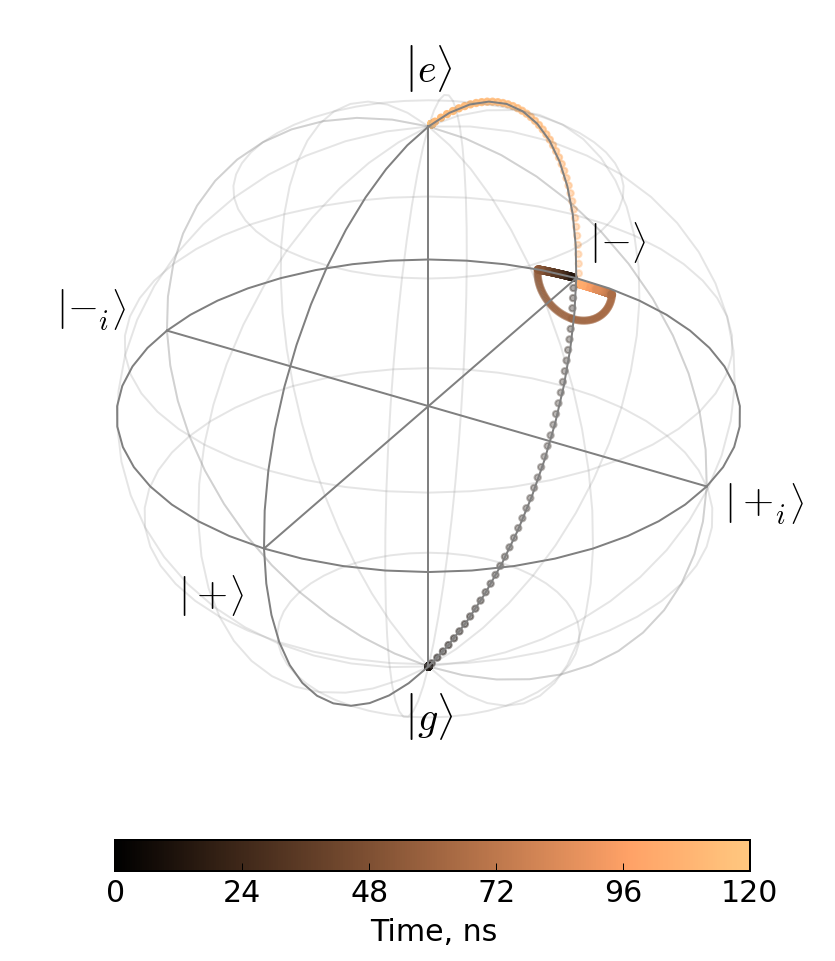
\includegraphics[width=0.9\textwidth]{cse_bloch_rf}
\caption{Schrödinger equation solution with driving and classical dephasing caused by the single $S(0)$ spectral component of the noise.}
\end{subfigure}
\begin{subfigure}[t]{0.45\textwidth}
\centering
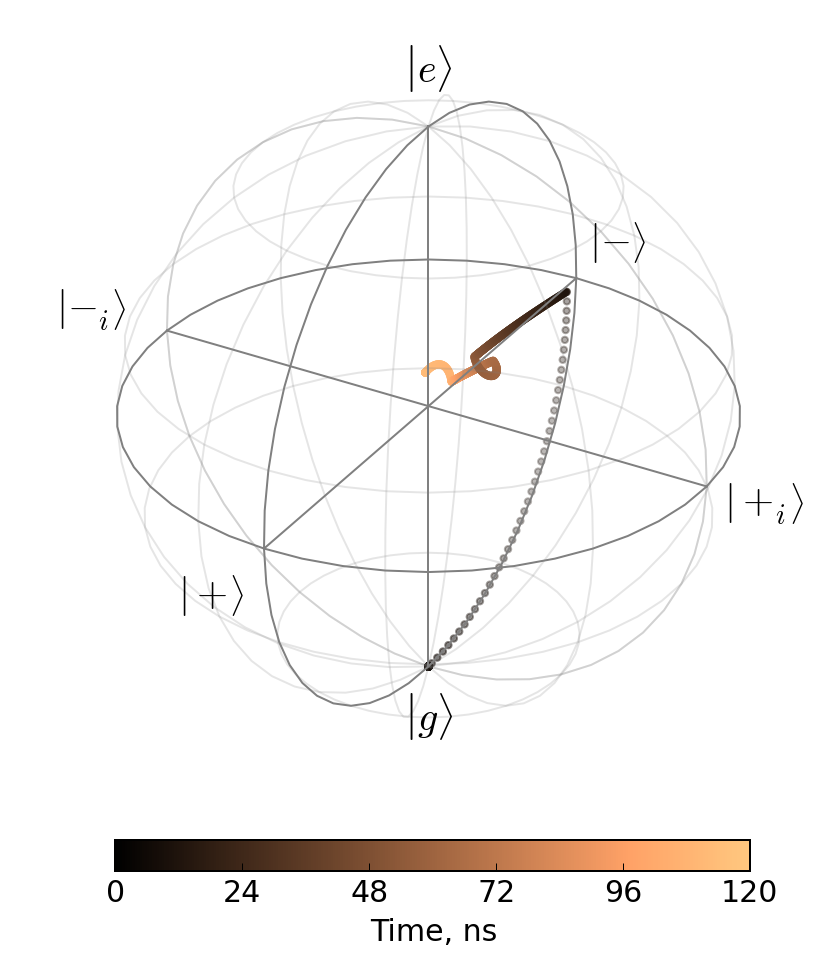
\includegraphics[width=0.9\textwidth]{qse_bloch_rf}
\caption{Master equation solution with driving and quantum dephasing.}
\end{subfigure}

\begin{subfigure}[t]{0.45\textwidth}
\centering
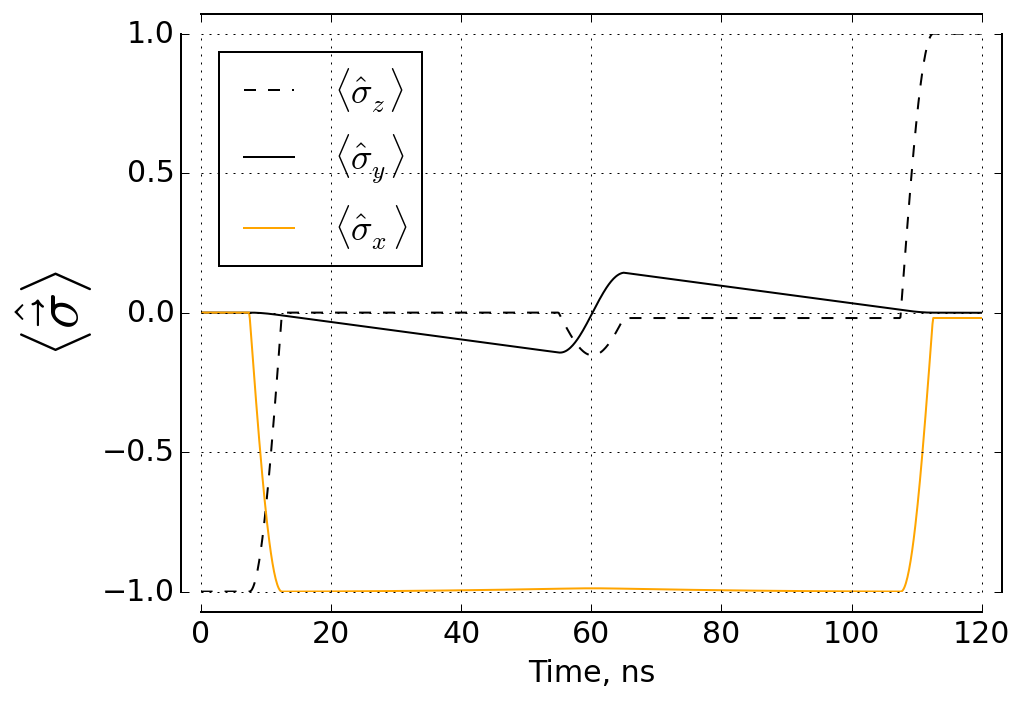
\includegraphics[width=0.99\textwidth]{cse_xyz_rf}
\caption{Same in $xyz$. Dephasing is linear in time and reversible for this case.}
\end{subfigure}
\begin{subfigure}[t]{0.45\textwidth}
\centering
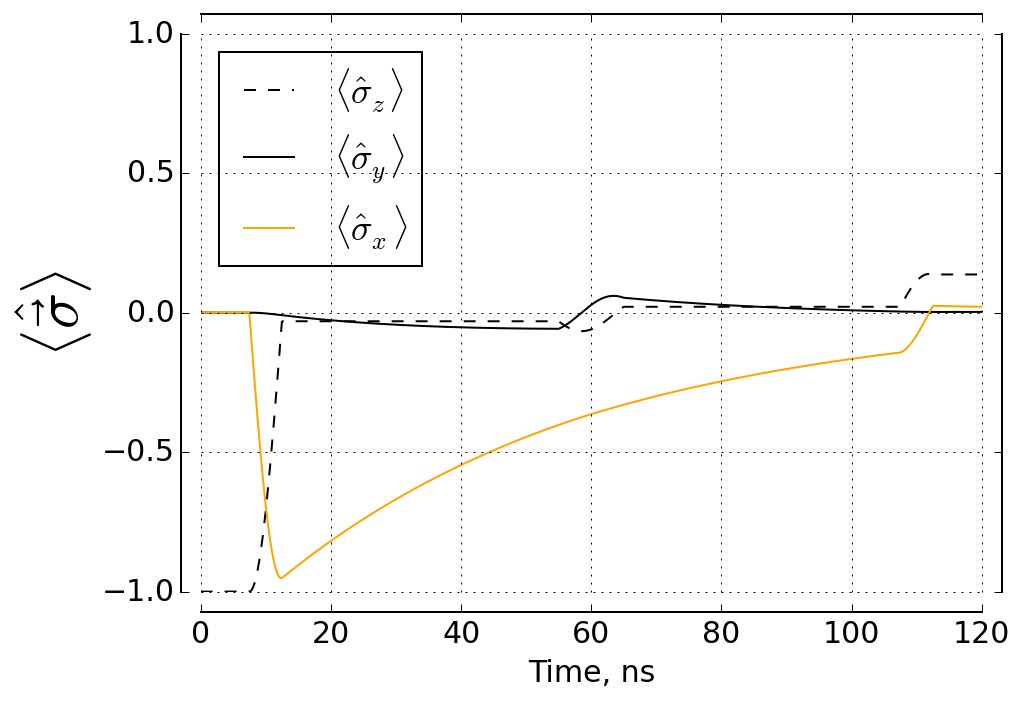
\includegraphics[width=0.99\textwidth]{qse_xyz_rf}
\caption{Same in $xyz$. Dephasing destroys the coherence and is irreversible.}
\end{subfigure}
\caption{Classical versus quantum spin-echo experiment modelling. Spin-echo can't cope with quantum noise.}
\label{fig:se}
\endgroup

\end{figure}

\bibliographystyle{ugost2008}
\bibliography{report.bib}
\end{document}